\documentclass[11pt,a4paper]{article}
%DIF LATEXDIFF DIFFERENCE FILE
%DIF DEL main_old.tex   Fri Apr 10 11:08:07 2026
%DIF ADD main_new.tex   Fri Apr 10 11:07:08 2026

% Packages
\usepackage[T1]{fontenc}
\usepackage{lmodern} % better fonts
\usepackage{microtype}
\usepackage[margin=1in]{geometry}
\usepackage{authblk}
\usepackage[round]{natbib}
\usepackage[hidelinks]{hyperref} % load before orcidlink
\usepackage{orcidlink}
\usepackage{amsmath}
\usepackage{amssymb}
 \usepackage{booktabs}
 \usepackage{multirow}
 \usepackage{graphicx}
\usepackage{subcaption}
\usepackage[ruled,vlined]{algorithm2e}

% Consistent math macros (optional but recommended)
\newcommand{\R}{\mathbb{R}}
\newcommand{\bx}{\mathbf{x}}
\newcommand{\by}{\mathbf{y}}
\newcommand{\E}{\mathbb{E}}
\newcommand{\SB}{\mathbf{S}_B}
\newcommand{\SW}{\mathbf{S}_W}


\title{Does Gradient Boosting improve with Fisher’s Discriminant analysis? Proposal of an integrated approach and empirical assessment of five popular datasets.}

\author[1]{Giulio Enzo Donninelli\thanks{Email: \href{mailto:g.donninelli@campus.unimib.it}{g.donninelli@campus.unimib.it} \quad ORCID: \orcidlink{0009-0009-7332-1159}}}
\author[1,2]{Pietro Giorgio Lovaglio\thanks{Email: \href{mailto:piergiorgio.lovaglio@unimib.it}{piergiorgio.lovaglio@unimib.it} \quad ORCID: \orcidlink{0000-0002-2340-0547}}}

\affil[1]{Dept of Statistics and Quantitative Methods, University of Milano-Bicocca, Milan, Italy}
\affil[2]{CRISP Research Center, University of Milano-Bicocca, Milan, Italy}

\date{} % omit date
%DIF PREAMBLE EXTENSION ADDED BY LATEXDIFF
%DIF CFONT PREAMBLE %DIF PREAMBLE
\RequirePackage{xcolor}\definecolor{RED}{rgb}{1,0,0}\definecolor{BLUE}{rgb}{0,0,1} %DIF PREAMBLE
\DeclareOldFontCommand{\sf}{\normalfont\sffamily}{\mathsf} %DIF PREAMBLE
\providecommand{\DIFaddtex}[1]{\textcolor{red}{#1}} %DIF PREAMBLE
\providecommand{\DIFdeltex}[1]{} %DIF PREAMBLE
%DIF SAFE PREAMBLE %DIF PREAMBLE
\providecommand{\DIFaddbegin}{} %DIF PREAMBLE
\providecommand{\DIFaddend}{} %DIF PREAMBLE
\providecommand{\DIFdelbegin}{} %DIF PREAMBLE
\providecommand{\DIFdelend}{} %DIF PREAMBLE
\providecommand{\DIFmodbegin}{} %DIF PREAMBLE
\providecommand{\DIFmodend}{} %DIF PREAMBLE
%DIF IDENTICAL PREAMBLE %DIF PREAMBLE
\providecommand{\DIFaddFL}[1]{\DIFadd{#1}} %DIF PREAMBLE
\providecommand{\DIFdelFL}[1]{\DIFdel{#1}} %DIF PREAMBLE
\providecommand{\DIFaddbeginFL}{\DIFaddbegin} %DIF PREAMBLE
\providecommand{\DIFaddendFL}{\DIFaddend} %DIF PREAMBLE
\providecommand{\DIFdelbeginFL}{\DIFdelbegin} %DIF PREAMBLE
\providecommand{\DIFdelendFL}{\DIFdelend} %DIF PREAMBLE
%DIF HYPERREF PREAMBLE %DIF PREAMBLE
\providecommand{\DIFadd}[1]{\texorpdfstring{\DIFaddtex{#1}}{#1}} %DIF PREAMBLE
\providecommand{\DIFdel}[1]{\texorpdfstring{\DIFdeltex{#1}}{}} %DIF PREAMBLE
%DIF COLORLISTINGS PREAMBLE %DIF PREAMBLE
\RequirePackage{listings} %DIF PREAMBLE
\RequirePackage{color} %DIF PREAMBLE
\lstdefinelanguage{DIFcode}{ %DIF PREAMBLE
%DIF DIFCODE_CFONT %DIF PREAMBLE
  moredelim=[il][\color{red}\scriptsize]{\%DIF\ <\ }, %DIF PREAMBLE
  moredelim=[il][\color{blue}\sffamily]{\%DIF\ >\ } %DIF PREAMBLE
} %DIF PREAMBLE
\lstdefinestyle{DIFverbatimstyle}{ %DIF PREAMBLE
	language=DIFcode, %DIF PREAMBLE
	basicstyle=\ttfamily, %DIF PREAMBLE
	columns=fullflexible, %DIF PREAMBLE
	keepspaces=true %DIF PREAMBLE
} %DIF PREAMBLE
\lstnewenvironment{DIFverbatim}{\lstset{style=DIFverbatimstyle}}{} %DIF PREAMBLE
\lstnewenvironment{DIFverbatim*}{\lstset{style=DIFverbatimstyle,showspaces=true}}{} %DIF PREAMBLE
%DIF END PREAMBLE EXTENSION ADDED BY LATEXDIFF

\begin{document}
\maketitle

\begin{abstract}
The aim of this study is to assess the impact of different dimensionality reduction techniques—specifically Principal Component Analysis (PCA) and Fisher's Linear Discriminant Analysis (LDA)—on the classification performance of Gradient Boosting Machines (GBM). While PCA is commonly employed to reduce feature dimensionality, often to speed up training or lower memory usage, its application is not standard in boosting pipelines. Moreover, to the best of our knowledge, no previous work has systematically explored whether LDA can enhance performance or is compatible with gradient boosting frameworks.\\[2ex]

In addition to evaluating the effects of PCA and LDA on the predictive performance of GBM, we introduce a novel integrated iterative algorithm that incorporates LDA-based feature transformation at each boosting step. Our analysis spans five classical benchmark datasets, representing diverse scenarios in terms of sample size, number of features, for both binary and multiclass targets. Results show that applying  \DIFaddbegin \DIFadd{LDA-derived }\DIFaddend features—and  \DIFaddbegin \DIFadd{in many settings the proposed LdaBoost integration}\DIFaddend — improves classification accuracy compared to standard GBM, particularly in multiclass settings or in binary problems with high feature dimensionality. Finally, through a set of controlled simulations, we investigate how the performance of the integrated approach evolves with increasing feature dimensionality and varying levels of feature correlation and sample size.

\end{abstract}

\section*{Statements}
\noindent\textbf{Data availability statement:} data are freely available online.\\
\textbf{Funding statement:} no funding received.\\
\textbf{Conflict of interest disclosure:} Authors have no conflicts of interest.

\newpage
\section{Introduction}
Real-world datasets often exhibit high dimensionality, which can hinder the performance of machine learning models. A common strategy to address this challenge is dimensionality reduction \citep{van2009dimensionality}. This involves transforming high-dimensional data into a more compact and informative representation, ideally one that reflects the data's intrinsic dimensionality \citep{huang2019review, bacanin2021dimensionality}.

Dimensionality reduction plays a critical role in machine learning by addressing the high dimensionality present in real-world data, thereby improving computational efficiency. By extracting the most informative features, it enables faster and more scalable algorithms---an essential advantage in real-time or resource-constrained applications.
Beyond computational gains, dimensionality reduction also mitigates the effects of the curse of dimensionality, which can significantly degrade model performance \citep{hu2024tackling}. For example, classification trees are prone to overfitting when trained on data with many irrelevant features, often resulting in higher missclassification rates on test sets.
In practice, dimensionality reduction not only reduces these risks but also facilitates the compression of high-dimensional data, ultimately supporting more accurate and efficient classification \citep{garcia2023evolutionary}.

Among the various data reduction techniques, feature extraction (FE) focuses on transforming the original feature space to generate new variables that form a more compact, lower-dimensional representation of the problem. Unlike unsupervised FE methods, supervised FE techniques aim not only to reduce dimensionality, but also to preserve class separability as much as possible \citep{fukunaga2013introduction}.
Common examples of unsupervised linear feature extraction methods include Principal Component Analysis (PCA) and Independent Component Analysis (ICA), which do not take class labels into account. In contrast, supervised methods such as Fisher's Linear Discriminant Analysis (LDA) and Partial Least Squares (PLS) explicitly incorporate class information to enhance discriminative power \citep{james2013introduction}.

Extending the first family of methods, manifold-based learning techniques aim to capture the nonlinear structure of the original data by uncovering its intrinsic local geometric properties. These approaches are based on the premise that the apparent high dimensionality of many datasets is often artificial \citep{zhou2011manifold}. Accordingly, they seek a lower-dimensional representation within a manifold---a topological space that is locally Euclidean---capable of preserving the underlying data structure.
Widely used examples include Locally Linear Embedding (LLE) \citep{roweis2000nonlinear}, Isometric Mapping (ISOMAP) \citep{tenenbaum2000global}, and Laplacian Eigenmaps (LE) \citep{belkin2003laplacian}. Another nonlinear approach that has gained popularity in recent years is the Autoencoder, which functions as an unsupervised multilayer perceptron for dimensionality reduction.
However, a major limitation of manifold learning methods is the lack of an explicit projection function, making them unable to handle new, unseen samples---commonly referred to as the out-of-sample problem \citep{bengio2003out}. This practical drawback helps explain the continued widespread use of linear feature extraction methods such as PCA, which offer both simplicity and robustness in real-world applications \citep{zebari2020comprehensive, sadegh2024comparative}.
A key limitation of PCA is that it identifies directions of maximum variance in the input space without regard to the target variable. As a result, the principal components may lack any discriminative power for classification tasks. Consistent with this, the literature has shown that supervised feature extraction methods generally outperform their unsupervised counterparts.
Among these, LDA is perhaps the most widely used supervised technique and has been shown to yield superior performance compared to PCA across a range of machine learning algorithms. This advantage stems from LDA's objective: it seeks linear combinations of the original predictors that maximize the separation between class means while minimizing within-class variance.
However, LDA comes with an inherent constraint: the number of extracted components is limited to $C - 1$, where $C$ is the number of classes. This is because LDA constructs a feature space optimized for discriminating among classes and thus only requires at most $C - 1$ dimensions to achieve optimal class separation. As a result, LDA can be viewed as an aggressive form of dimensionality reduction, compressing the original $p$-dimensional predictor space into a space of at most $C - 1$ dimensions. In the extreme case of a binary classification problem ($C = 2$), LDA produces only a single discriminant component.

In empirical studies comparing different feature extraction (FE) strategies, the classifiers used are often limited to traditional models such as logistic regression, classification trees, k-nearest neighbors (KNN), or Na\"ive Bayes. However, these models are rarely applied in real-world classification tasks due to their relatively limited performance compared to ensemble methods like Random Forest (RF) or Gradient Boosting Machines (GBM) \citep{fernandez2014we,  chen2016xgboost}.
GBM is an iterative algorithm that combines multiple weak learners---typically shallow classification trees---into a strong predictive model. Each weak learner is trained to minimize the loss function of the previous ensemble using gradient descent. The learners are built sequentially, with each iteration aiming to model the residuals (errors) of the previous stage. This process continues iteratively, where each new learner corrects the mistakes of its predecessors, progressively improving overall model accuracy.

Extreme Gradient Boosting (XGBoost, \cite{chen2016xgboost}) is a widely used implementation of GBM, known for its speed and strong performance in both applied settings and machine learning competitions. XGBoost incorporates regularization techniques and additional strategies---such as random selection of features for each weak learner---to mitigate overfitting.
However, studies on preprocessing for GBM and XGBoost remain limited, typically focusing on standard procedures such as missing value imputation, outlier handling, and managing high collinearity or near-zero variance in input features \citep{gabriel2023optimizing, chen2016xgboost}.
While not standard, the use of PCA prior to gradient boosting has not been extensively studied in the literature and is primarily mentioned in the context of machine learning competitions (such as the KDD Cup or Kaggle) as a heuristic to reduce feature dimensionality and, in some cases, to accelerate training or reduce memory consumption \citep{rakhshan2020tensorized}.
In contrast, to the best of our knowledge, no existing study has explored the use of LDA in conjunction with GBM. Specifically, there is no established practice or empirical evidence suggesting that LDA enhances performance or is compatible with gradient boosting models. In this respect, it is perhaps unsurprising that LDA has not been incorporated as a preprocessing step in widely used automated machine learning (AutoML) frameworks \citep{NIPS2015_11d0e628}.

The aim of this paper is twofold. First, it investigates the impact of feature extraction via PCA and LDA on the classification accuracy of the GBM algorithm. Second, in contrast to common approaches that apply machine learning models to a fixed set of preprocessed features, we propose an integrated iterative method that leverages LDA-based feature transformation at each stage of the GBM training process. This integration acknowledges the iterative nature of GBM, where the target variable is updated at each step as the residual of the previous weak learner. The resulting algorithm, which we refer to as LdaBoost, dynamically recalculates LDA projections throughout boosting iterations.
The rationale behind this approach lies in the complementary strengths of LDA and GBM. While LDA projects data onto a lower-dimensional linear subspace that maximally separates the classes, the resulting projections serve as informative inputs for GBM, which constructs nonlinear decision boundaries through ensembles of shallow trees. For instance, in a three-class problem, LDA maps observations into a two-dimensional space where the classes form compact and well-separated clusters---structures that GBM can efficiently capture using combinations of simple, rectangular tree splits. This synergy is particularly beneficial in complex classification tasks where linear separability is insufficient on its own.
\DIFaddbegin \DIFadd{From a boosting perspective, LdaBoost is conceptually related to variants that modify the boosting geometry through margin constraints, filtering, or projection mappings (for example LPBoost, FilterBoost, and projection/kernel-based boosting variants). The key difference is that LdaBoost recomputes a supervised linear projection inside each boosting round from the current multinomial gradients, and then fits class-wise trees in this stage-specific projected space. In this sense, the projection update is part of the boosting loop itself rather than an external preprocessing step.
}\DIFaddend To address both research objectives, we conduct a series of experiments on several classical benchmark datasets that cover a variety of scenarios in terms of sample size, feature dimensionality, and target type (binary and multiclass). We compare the classification performance of standard GBM with and without dimensionality reduction, applying PCA, LDA, and the proposed LdaBoost algorithm. The results show that incorporating LDA-based features substantially enhances GBM accuracy, with the integrated LdaBoost method yielding the most consistent and significant improvements over the baseline.
In addition, we explore how the performance of LdaBoost varies with key data characteristics, specifically the number of observations, input features and their average correlation. Using simulations, we examine these effects systematically, offering insights into the conditions under which LdaBoost is most beneficial also in comparison with the optimal Bayes classifier. To the best of our knowledge, this is the first study to investigate the integration of LDA within a gradient boosting framework.

The remainder of the paper is structured as follows: Section~2 reviews related work on feature extraction in machine learning, with a focus on PCA and LDA. Section~3 introduces the LdaBoost algorithm in detail. Section~4 describes the analysis framework and datasets used. Section~5 presents the main empirical findings, including results from the simulation study. Finally, Section~6 concludes the paper by summarizing the contributions and outlining directions for future research.


\section{Related Work}
Many authors have attempted to evaluate how feature extraction methods perform in classification tasks. Zebari et al. \citep{zebari2020comprehensive} provide an excellent review in this regard.  
The authors reviewed 21 feature extraction methods from the literature. Among them, eight methods relied on PCA, while seven were based on Deep Neural Network (DNN) and Convolutional Neural Network (CNN) tools, some of which were integrated with autoencoders or PCA.  
Other approaches aimed at dimensionality reduction used specific techniques for extracting features from machinery signals, such as Fourier transform frequency spectrum, envelope analysis, and local mean decomposition. Additionally, methods specific to image analysis adopted texture feature extraction and wavelet transformations.

Most of the reviewed approaches are unsupervised FE methods, with some exceptions that integrate PCA or autoencoders with supervised DNN and CNN architectures used as wrapper feature extraction tools. Specifically, both semi-supervised algorithms select the most optimal features (neurons from hidden layers or image features from convolutional layers) based on the performance of the learning algorithm aimed at predicting the target variable.  
Here, PCA was not used to extract the initial features for DNN and CNN but rather to reduce the dimensionality of the extracted features (neurons) from both neural network tools.  
The findings demonstrated the efficacy of semi-supervised dimensionality reduction techniques in improving the performance of machine learning algorithms compared to unsupervised tools (essentially PCA).  
However, no study has used LDA as a feature extraction method.

In the above-cited review, the SVM algorithm was the most frequently used classifier in conjunction with feature extraction, followed by neural networks, KNN, and LDA.  
The conclusion is that optimized PCA (within a semi-supervised approach) achieves better performance in terms of accuracy, computational time, and the number of reduced features \citep{ma2019dimension, zebari2020comprehensive}.  
Apart from a few exceptions, however, classifiers used in the literature rarely include tree-based ensembles such as Random Forest (RF) or Bagging, and none of them incorporate GBM.

As mentioned, only a few published studies have adopted LDA as a feature extraction method.  
Subasi \citep{subasi2010eeg} classified epileptic seizures using EEG signals and an SVM classifier. The classification rate with LDA feature extraction was the highest (100\%), followed by ICA (99.5\%), while PCA achieved the lowest correct classification rate (98.75\%).  
All FE strategies performed better than classification without feature extraction (98\%). Moreover, the proposed FE strategies outperformed the overall classification accuracy obtained using a Mixture of Experts model (94.5\%) and an Artificial Neural Network (93.2\%).

Leo et al. \citep{leo2014efficient}, using a chemical sensor array dataset, fitted an SVM classifier with dimensionality reduction methods PCA and LDA. The authors demonstrated that LDA better separated the data to be classified, resulting in higher accuracy.

Data from Human Activity Recognition (HAR), aimed at identifying human activity based on attributes measured by a smartphone's accelerometer and gyroscope, were also used to assess machine learning tools in conjunction with feature preprocessing.  
In this field, using the Human Activity Recognition Using Smartphones Data Set (UCI Machine Learning Repository), Luštrek and Kaluža \citep{luvstrek2009fall} evaluated various algorithms (including C4.5 decision trees) using cross-validated classification accuracy.

Cann \citep{cannfeature}, applying the C4.5 classification decision tree algorithm with LDA, found that such feature preprocessing increased accuracy by 1.61\% compared to using the original inputs.

Pechenizkiy et al. \citep{pechenizkiy2006combining} proposed a novel feature extraction method combining two steps: first extracting principal components and then deriving discriminant components from the resulting PCA feature space.  
However, this combined approach introduces some arbitrariness, as the discriminant components (scores) depend on the initial number of extracted principal components.  
Yang \citep{yang2003can} recommends using more PCA dimensions to improve the performance of discriminant components in the second step.

These authors assessed KNN, Naïve Bayes, and C4.5 decision tree algorithms on 21 datasets.  
Although specific improvements depended on the dataset, combining LDA and PCA generally showed an overall increase in accuracy compared to using PCA or LDA alone, though the improvement over LDA was less pronounced.  
Li \citep{li2009face} applied the same combined approach for face recognition using the nearest neighbor classifier and observed improved results compared to PCA alone.

Liu et al. \citep{liu2019discriminative}, analyzing numerous public image datasets, developed a method for feature extraction based on combining discriminant analysis with the low-rank representation (LRR) of the original data samples.  
In particular, LDA was used as a discriminative constraint term within the dimensionality reduction loss function, which was minimized with respect to the lowest-rank representation of the original data.  
A projection matrix was simultaneously learned for dimensionality reduction and class separation.  
The global subspace structure of the original samples was first captured by LRR, and then the discriminative constraint term was used to maximize the between-class distances and minimize the within-class distances in the low-dimensional projection space.

The authors demonstrated that the proposed strategy achieved better recognition accuracy compared to state-of-the-art feature extraction methods.  
Although the proposed supervised FE method was specifically designed for image processing, this approach illustrates that integrating discriminant analysis with supervised classifiers can be beneficial in terms of predictive accuracy.



\section{Methods}


Given  \DIFaddbegin \DIFadd{training features $(x_1, \dots, x_N)$, with }\DIFaddend $x_i \in \mathbb{R}^p$ \DIFaddbegin \DIFadd{, PCA is defined without using class labels. For supervised methods introduced later, we denote labels by $y_i \in \{1,\dots,C\}$.  
}\DIFaddend 

PCA maps the feature space $x_i \in \mathbb{R}^p$ to a lower-dimensional space $t_i \in \mathbb{R}^r$ ($r \leq p$) through a linear transformation:
\[
t_i = P^\top x_i
\]
(Principal component scores), where these new $r$ variables are uncorrelated.

The PCA criterion aims to maximize the sum of variances (trace) of the retained $r$ principal component scores, e.g. $\text{trace}(P^\top S P)$, where $P^\top S P$ is the covariance matrix of the principal component scores and $S$ is the covariance matrix of the original features $S = X^\top X$.  
This is achieved by selecting the $r$ largest eigenvalues of $S$, and the corresponding eigenvectors $P_1, \dots, P_r$ form the optimal transformation matrix:
\[
P = [P_1 \ | \dots | \ P_r].
\]

LDA maps the feature space $x_i \in \mathbb{R}^p$ to a lower-dimensional space $q_i \in \mathbb{R}^r$ ($r < p$) through a linear transformation:
\[
q_i = G^\top x_i.
\]
Discriminant scores are weighted linear combinations of the predictors.  
The weights are estimated to maximize the differences between class mean discriminant scores and are obtained as generalized eigenvectors that maximize the ratio of the between-class sum of squares ($S_B$) to the within-class sum of squares ($S_W$).  
The former evaluates the spread of the class means ($\mu_c$) around the global mean ($\mu$), whereas the latter evaluates the spread of the data ($x_i$) around the class mean ($\mu_c$).

For transformed data, the (transformed) within-class and between-class sums of squares are defined respectively as $G^\top S_W G$ and $G^\top S_B G$.  
The LDA optimization problem requires minimizing the transformed within-class scatter while maximizing the transformed between-class scatter.  
The optimal transformation $G$ can be obtained by maximizing the Fisher criterion:
\[
\frac{|G^\top S_B G|}{|G^\top S_W G|}
\]
by selecting the $r$ largest eigenvalues of $S_W^{-1} S_B$ and the corresponding eigenvectors $G_1, \dots, G_r$, which form the optimal transformation matrix:
\[
G = [G_1 \ | \dots | \ G_r].
\]
 \DIFaddbegin \DIFadd{Hence, the discriminant weights depend jointly on between-class mean separation and within-class variability (including covariance): a feature receives a larger coefficient only when it contributes to class separation relative to its within-class dispersion}\DIFaddend .

Hence, LDA provides new $N$ training data $(q_1, y_1(c)), \dots, (q_N, y_N(c))$, where $q_i \in \mathbb{R}^r$ are the input $r$ variables retained after LDA computation (discriminant components).

---

Concerning the Gradient Boosting classifier, we use the classical GBM \citep{friedman2001greedy} implemented in the Python library \texttt{GradientBoostingClassifier} within Scikit-learn.  

GBM builds an additive model in a forward stage-wise fashion using classification trees.  
In each stage (\texttt{n\_estimators}), trees are fit on the negative gradient of the loss function, which is either the binary log-loss (binomial deviance) or the multiclass log-loss (the multinomial negative log-likelihood loss function) for multi-class classification with \texttt{n\_classes} mutually exclusive classes.

The GBM is an additive model whose prediction $\hat{y}_i$ for a given input $x_i$ is defined as:
\[
\hat{y}_i = F_M(x_i) = \sum_{m=1}^M h_m(x_i) \tag{1}
\]
where $h_m$ is estimated by the $m$-th tree, and $M$ is the maximum number of trees used.  
GBM proceeds in a greedy fashion:
\[
F_m(x) = F_{m-1}(x) + h_m(x),
\]
where, at iteration $m$, a newly added tree $h_m$ is fitted to minimize a sum of losses $L_m$, given the previous ensemble $F_{m-1}(x)$:
\[
h_m = \arg \min_h L_m = \arg \min_h \sum_{i=1}^n \ell \Big(y_i, F_{m-1}(x_i) + h(x_i)\Big). \tag{2}
\]

Moreover, GBM allows a regularization strategy that scales the contribution of each weak learner by a constant factor $\nu$ (\texttt{learning\_rate}):
\[
F_m(x) = F_{m-1}(x) + \nu h_m(x).
\]
At each iteration, the estimator $h_m(x)$ is fitted to predict the negative gradients of the samples.

The iterative minimization of the loss function is achieved by Gradient Descent, using all instances in each iteration or a subsample of observations for fitting the individual trees (Stochastic or Batch Gradient Descent).

The main tuning parameters for GBM are:  
- the learning rate (\texttt{learning\_rate}),  
- the maximum number of trees (\texttt{n\_estimators}),  
- the maximum number of final nodes in each tree (\texttt{max\_depth}),  
- the minimum number of observations in final nodes (\texttt{min\_samples\_leaf}),  
- and the percentage of observations used in each stochastic gradient descent iteration (\texttt{subsample}).


\subsection{An integrated LdaBoosting algorithm}
The key insight behind integrating LDA within the GBM algorithm—referred to as \textbf{LdaBoost}—is to dynamically leverage the discriminative power of LDA at each iteration of the boosting procedure.  
Traditionally, LDA is employed as a pre-processing step to reduce feature dimensionality by projecting the original feature space onto a subspace optimized for class separability.  
However, this static approach neglects the iterative nature of GBM, wherein the target changes at each step as the model seeks to correct residual errors from the preceding weak learner.

In contrast, LdaBoost iteratively updates the feature projections using LDA based on the residuals produced at each boosting round, thereby continuously refining the feature space in alignment with the evolving predictions.  
 \DIFaddbegin \DIFadd{For $m>0$, let
}\[
\DIFadd{g^{(m)}_{i,c} = Y_{i,c} - P^{(m-1)}_{i,c}, \qquad
z^{(m)}_i = \arg\max_{c\in\{1,\dots,C\}} g^{(m)}_{i,c},
}\]
\DIFadd{where $Y$ is one-hot encoded and $P^{(m-1)}$ are current class probabilities. We then fit LDA on $(X, z^{(m)})$ and obtain $G^{(m)}$ by maximizing the Fisher ratio
}\[
\DIFadd{\max_G\ \frac{|G^\top S_B(z^{(m)})G|}{|G^\top S_W(z^{(m)})G|}.
}\]
\DIFadd{Therefore, Step 1 remains a valid Fisher optimization at each round because it is always solved on a well-defined categorical partition; the partition itself is updated by boosting gradients. In case of ties in the $\arg\max$, we adopt the deterministic first-index rule. If provisional labels collapse to fewer than two classes, we reuse the previous valid projection to keep the stagewise update well-defined}\DIFaddend .  
This iterative integration not only capitalizes on LDA’s capacity to enhance linear class separation but also synergistically complements GBM’s nonlinear modeling strengths, resulting in improved classification accuracy.  

The pseudocode, illustrated in Box 1, summarizes the LdaBoost procedure, clarifying the step-by-step algorithmic implementation of this integrated approach, as follows:

\begin{itemize}
    \item \textbf{Initialization.} One-hot encode labels $Y$ and estimate empirical class priors $\hat{\pi}_c$; initialize logits with $F^{(0)}_c = \log \hat{\pi}_c$ so boosting starts from the log prior odds shared by all samples.

    \item \textbf{Step 1 – Iteration-specific LDA transform.} At $m=0$, fit LDA on true labels $y$ to get projection $G^{(0)}$ and discriminant scores $Q^{(0)}$ (each $q_i = G^{(0)\top} x_i$) in an $r \le C-1$ subspace that maximizes between-class separation.  
    For $m>0$, form current probabilities $p^{(m-1)}$, gradients $g^{(m)} = Y - p^{(m-1)}$,  \DIFaddbegin \DIFadd{and induced labels $z_i^{(m)}=\arg\max_c g^{(m)}_{i,c}$ (deterministic tie-breaking). Refit LDA on $(X,z^{(m)})$ }\DIFaddend to obtain $G^{(m)}$ \DIFaddbegin \DIFadd{; if $z^{(m)}$ contains fewer than two classes, reuse $G^{(m-1)}$}\DIFaddend .

    \item \textbf{Step 2 – Pseudo-residuals.} Recompute $g^{(m)} = Y - p^{(m-1)}$; these are the negative gradients of the multinomial deviance with respect to the logits and provide the working response for the boosted trees.

    \item \textbf{Step 3 – Class-wise weak learners.} Train one regression tree per class $c$ to predict the corresponding gradient column $g^{(m)}_{\cdot,c}$ from the current discriminant scores $Q^{(m)}$; using the LDA subspace concentrates each tree on directions most informative for class separation at round $m$.

    \item \textbf{Step 4 – Stagewise update.} Update additive logits:
    \[
    F^{(m)}_{i,c} = F^{(m-1)}_{i,c} + \nu \, h_{m,c}\left(Q^{(m)}_i\right),
    \]
    where the learning rate $\nu$ (shrinkage) scales each correction, as in standard gradient boosting.

    \item \textbf{Class prediction.} Start from $F^{(0)}$; for each stage, apply stored $G^{(m)}$ to a new $x$ to get $q$, add $\nu \, h_{m,c}(q)$ to each class logit, then apply the softmax to obtain probabilities and choose the class with the maximum value.
\end{itemize}

\begin{algorithm}[h!]
\caption{LdaBoost (multiclass)}
\KwIn{Training data $(\bx_i,y_i)_{i=1}^N$, classes $\{1,\dots,C\}$, rounds $M$, learning rate $\nu$}
\KwOut{Additive logits $F^{(M)}$ and per-round projections $\{G^{(m)}\}_{m=0}^{M-1}$}

\textbf{Init:} One-hot $Y\in\{0,1\}^{N\times C}$, priors $\hat\pi_c$, $F^{(0)}_{i,c}\gets \log\hat\pi_c$,
$P^{(0)}=\mathrm{softmax}(F^{(0)})$. Fit $G^{(0)}$ via LDA on  \DIFaddbegin \DIFadd{$(X,y)$}\DIFaddend ; set $Q^{(0)}=X G^{(0)}$.

 \DIFaddbegin \For{$m=1$ \KwTo $M$}{
  $R^{(m)} \gets Y - P^{(m-1)}$ \tcp*{negative gradients of multinomial deviance}
    $z^{(m)}_i\gets \arg\max_c R^{(m)}_{i,c}$ for each $i$;\\
    \eIf{$z^{(m)}$ has at least two classes}{
        Refit $G^{(m)}$ via LDA on $(X,z^{(m)})$;
    }{
        $G^{(m)}\gets G^{(m-1)}$;
    }
  $Q^{(m)} \gets X G^{(m)}$;\\
  \For{$c=1$ \KwTo $C$}{
    Fit regression tree $h_c^{(m)}: Q^{(m)}\to R^{(m)}_{\cdot,c}$;
  }
  $F^{(m)}_{\cdot,c} \gets F^{(m-1)}_{\cdot,c} + \nu\, h_c^{(m)}(Q^{(m)})$ for all $c$;\\
  $P^{(m)}\gets \mathrm{softmax}(F^{(m)})$.
}
\DIFaddend \textbf{Predict:} Apply $\{G^{(m)}\}$ and $\{h_c^{(m)}\}$ sequentially to a new $\bx$; return $\arg\max_c F^{(M)}_c$.
\end{algorithm}

\DIFaddbegin \subsection*{\DIFadd{Computational scalability}}
\DIFadd{Let $n$ be the number of samples, $p$ the number of features, $C$ the number of classes, and $M$ the number of boosting rounds. A one-shot LDA+GBM pipeline fits LDA once and then trains $M$ boosting stages on fixed transformed features. By contrast, LdaBoost recomputes LDA at each round.
}

\DIFadd{Denoting by $\mathcal{C}_{\mathrm{LDA}}(n,p,C)$ the cost of one LDA fit and by $\mathcal{C}_{\mathrm{tree}}(n,C)$ the cost of one class-wise boosting stage, the overall costs are:
}\[
\DIFadd{\text{LDA+GBM: } \mathcal{C}_{\mathrm{LDA}}(n,p,C) + M\,\mathcal{C}_{\mathrm{tree}}(n,C),
}\]
\[
\DIFadd{\text{LdaBoost: } M\,\mathcal{C}_{\mathrm{LDA}}(n,p,C) + M\,\mathcal{C}_{\mathrm{tree}}(n,C).
}\]
\DIFadd{Thus, the additional overhead of LdaBoost is approximately $(M-1)\,\mathcal{C}_{\mathrm{LDA}}(n,p,C)$ relative to one-shot LDA preprocessing. In practice, this trade-off is more visible in high-dimensional settings, where repeated scatter-matrix computations dominate runtime, and is much smaller when $p$ is modest.
}


\DIFaddend \section{Dataset and Empirical Strategy}
From an empirical perspective, the assessment of algorithms (GBM in PCA/LDA framework) can be summarized as follows:

\begin{itemize}
    \item \textbf{Step 1.} The features were normalized to have values in the range $[0,1]$.

    \item \textbf{Step 2.} Features were extracted using the PCA (principal components) and LDA (discriminant components) algorithms to reduce dimensionality.  
    For situations where both training and test sets are available, both datasets were transformed using PCA and LDA.  
    For the test set, the principal and discriminant scores were calculated using the training weights.

    \item \textbf{Step 3.} The classification process for each dataset was carried out using GBM-based classification on:
    \begin{itemize}
        \item normalized original features,
        \item PCA-based features (\textbf{PCA+GBM}),
        \item LDA-based features (\textbf{LDA+GBM}).
    \end{itemize}

    \item \textbf{Step 4.} The proposed \textbf{LdaBoost} model was also fitted for each dataset.
\end{itemize}


\subsection*{Datasets}
The Human Activity Recognition Using Smartphones dataset (UCI Machine Learning Repository). The dataset has 6 balanced class labels representing the following conditions: 1 WALKING, 2 WALKING\_UPSTAIRS, 3 WALKING\_DOWNSTAIRS, 4 SITTING, 5 STANDING, 6 LAYING.

The dataset contains 10,299 observations and 561 features recorded from a waist-mounted smartphone with inertial sensors. The data from the UCI Machine Learning Repository are already normalized (within [-1, 1]) and  \DIFaddbegin \DIFadd{reported }\DIFaddend in a 0-1 range. Data were split into training and test sets. Both test accuracy and cross-validated accuracy were evaluated.

Iris dataset (UCI Machine Learning Repository). The dataset consists of 50 samples from each of three species of Iris (Iris setosa, Iris virginica, and Iris versicolor). Four features were measured from each sample: the length and the width of the sepals and petals, in centimetres. Features were normalized. Data were not split, and the cross-validated accuracy was evaluated.

Sonar dataset (UCI Machine Learning Repository). The data contain patterns obtained by bouncing sonar signals off a metal cylinder at various angles and under various conditions. Each pattern is a set of numbers in the range 0.0 to 1.0. Each number represents the energy within a particular frequency band, integrated over a certain period of time. The label associated with each record is “R" if the object is a rock and "M" if it is a mine (metal cylinder). The data have 60 features and 208 observations. Features are already normalized. Data were not split, and the cross-validated accuracy was evaluated.

Yeast dataset (Kaggle Repository). The Yeast dataset consists of a protein-protein interaction network. The target has 10 unbalanced classes, indicating the localization site of the protein (e.g., cytosolic or cytoskeletal, nuclear, extracellular, etc.). The data contain 8 features and 1,484 observations. Features were normalized. Data were not split, and the cross-validated accuracy was evaluated.

Rainfall Dataset (Kaggle Repository). This dataset collects a time series of 2,919 observations (days) regarding weather conditions, meteorological variables, and rainfall. The target (rainfall) is binary, and there are 11 features summarizing atmospheric conditions (humidity, sunshine, wind direction, wind speed, etc.). Features were normalized. Data were split, and both test accuracy and cross-validated accuracy were evaluated.



\subsection*{Tuning strategy}
Firstly, using normalized inputs, we fit a classical GBM with \texttt{GradientBoostingClassifier} of Scikit-Learn Python library.
We tune, using 10-fold cross-validation, the following parameters:  \texttt{max\_depth}, \texttt{n\_estimators}, and \texttt{min\_samples\_leaf}, fixing \texttt{learning\_rate} at 0.05 and the number of observations for each stochastic gradient descent iteration (\texttt{subsample}) at 0.6 as reasonable values for all algorithms.

Secondly, to assess how the performance of different algorithms depends only on the utilized features, the best-tuned parameters of GBM were also used for PCA+GBM, LDA+GBM, and LdaBoost. Specifically, for PCA+GBM, we also tune the optimal number of principal components (maximizing the cross-validated accuracy), whereas for both LDA+GBM and LdaBoost, we retain the maximum number of discriminant scores (\#classes$-1$).

Thirdly, only for LdaBoost do we refit the algorithm (\texttt{LdaBoost\_tuned}), this time also tuning the parameters — \texttt{max\_depth}, \texttt{n\_estimators}, and \texttt{min\_samples\_leaf} — which were previously fixed to match the GBM estimates for ease of comparison. This allows us to assess whether LdaBoost's accuracy benefits from full and unconstrained parameter tuning.

 \DIFaddbegin \DIFadd{This design intentionally prioritizes a transformation-focused comparison, but it also introduces asymmetries that should be made explicit. In particular, GBM hyperparameters are optimized in the original feature space and then reused for PCA+GBM, LDA+GBM, and fixed-parameter LdaBoost, so part of the observed gap may reflect suboptimal retuning in transformed spaces. For this reason, we report \texttt{LdaBoost\_tuned} separately and interpret fixed-parameter comparisons as controlled feature-space contrasts rather than fully optimized head-to-head rankings.
}

\DIFadd{Likewise, PCA is tuned over the number of retained components, whereas LDA-based pipelines retain the theoretical maximum of $C-1$ discriminant scores. This choice follows the Fisher-LDA construction, but it is another source of asymmetry; an ablation over reduced LDA dimensionality is therefore a relevant extension for future work.
}

\DIFadd{Finally, beyond reporting means and standard deviations, we ran nonparametric significance checks on the simulation comparison outputs using matched replicate-setting blocks. Specifically, for each target scenario (binary/ternary/quinary at $N=1{,}000$) we applied a Friedman test across the three pipelines and paired Wilcoxon signed-rank tests for pairwise contrasts on aggregated blocks ($5$ feature settings $\times$ $5$ replications, $n=25$). The Friedman p-values were 0.302 (binary), 0.073 (ternary), and 0.338 (quinary), indicating no global difference at the 0.05 level; after Holm correction across pairwise Wilcoxon contrasts, no pairwise comparison remained significant at 0.05. These checks are therefore reported as robustness diagnostics and should be interpreted together with effect sizes and descriptive variability.
For the real-dataset analyses, the cross-validation configuration was 10 folds for HAR, IRIS, SONAR, and Rainfall, and 5 folds for YEAST, with sample sizes of 7,352 (HAR train, plus 2,947 external test), 150 (IRIS), 208 (SONAR), 2,190 (Rainfall train, plus 730 external test), and 1,484 (YEAST). These values define the fold/sample context for the reported means and standard deviations; however, fold-level paired score vectors were not archived as a unified real-data artifact in the current release, so fully paired inferential tests on all real datasets remain future work.
}

\DIFadd{For each }\DIFaddend dataset, algorithms were compared using 10-fold cross-validated accuracy, and for the HAR and Rainfall datasets, also by test accuracy (for HAR we use the test set available from UCI  \DIFaddbegin \DIFadd{Machine Learning}\DIFaddend ). 
For the HAR dataset, we also evaluate the macro F1 score as  \DIFaddbegin \DIFadd{an }\DIFaddend accuracy measure for a more complete assessment.


\subsection*{LdaBoost Simulations}
To comprehensively evaluate the robustness and performance of the proposed LdaBoost algorithm, we conducted a series of simulations to explore how classification accuracy varied across different scenarios. Specifically, we systematically assessed the influence of three critical factors: the number of observations,the number of features and the degree of correlation among these features.

In these simulations, synthetic datasets of 1,000 and 10,000 observations were generated using a multivariate normal distribution, $X \sim \mathcal{N}(\mu_y, \Sigma)$, with mean vectors $\mu_y$ set distinctly for each class and type of target (see below). The covariance matrix $\Sigma$ was generated using a symmetric structure with diagonal elements equal to 1, and off-diagonal elements sampled from a truncated normal distribution with a mean of 0.5 and a standard deviation of 1, ensuring correlations within a realistic range between -1 and 1.

Additionally, correlation levels among features were manipulated through the covariance matrix, simulating conditions ranging from weak to strong correlations. Particularly, the mean correlation ($\rho$) of non-diagonal elements of $\Sigma$ was considered, and representative values of $\rho = 0.0$, $0.2$, $0.5$ and $0.7$ were simulated . 

\textbf{To construct the target variable $Y$, two distinct scenarios were considered:}

\begin{itemize}
    \item \textbf{Binary scenario:} Two distinct class-specific mean vectors, $\mu_0=0$ and $\mu_1=1$, were established. Observations were generated from multivariate densities (f) as follows:
    \[
    f(X|Y=0) \sim \mathcal{N}(0,\Sigma), \quad f(X|Y=1) \sim \mathcal{N}(1,\Sigma)
    \]
    The class labels were determined based on which Gaussian distribution each observation originated from.

    \item \textbf{Multiclass scenario:} Multiple distinct mean vectors $\mu_c = c$ were carefully defined to maximize nonlinear separability. Observations were generated as:
    \[
    f(X|Y=c) \sim \mathcal{N}(\mu_c,\Sigma),\quad \mu_c=c, \quad c = 1,2,\dots,C\
    \]
    Each observation's class label was directly assigned according to the Gaussian distribution from which it was drawn. In simulation, for multiclass target we use both C= 3 and C=5.
\end{itemize}

These simulated distributions provide a moderate to high class overlapping in the feature space, thus avoiding linear separability or clear class separation. Moreover, the use of normal likelihoods makes the Bayes classifier — based on Bayes' Theorem — computationally feasible. The Bayes classifier (assuming equal priors) was fitted to each simulated dataset, and its resulting accuracy — representing the theoretical upper bound or ideal performance achievable — was used as a benchmark when evaluating LdaBoost simulations.
The number of features was systematically varied at distinct levels (5, 50, 100, 300, and 400) to represent scenarios ranging from low to very high dimensionality. 

For each scenario (sample size, number of features and $\rho$) we generate random samples (realizations) from the assumed distribution in order to exploit Monte Carlo variability of accuracies (with standard deviation, SD). 
In the analysis of the real dataset, SD denotes the cross-validated standard deviation, while accuracy, unless otherwise specified, refers to cross-validated accuracy.
Two complementary simulation campaigns were performed. The first compared GBM, PCA+GBM, LDA+GBM, and LdaBoost (Figures~\ref{fig:fig1}--\ref{fig:fig2}--A7--A8--A9). 
The second evaluates LdaBoost across scenarios, benchmarking it against the Bayes classifier (Figures~\ref{fig:fig3}--\ref{fig:fig4}--\ref{fig:fig5}--\ref{fig:fig6}). This design highlights how closely the proposed method can approach the theoretical upper bound across heterogeneous data-generating processes.

\DIFaddbegin \DIFadd{At the same time, we acknowledge that these simulations rely on multivariate normal generators with class-specific means, a setting that is favorable to LDA-type projections and therefore may overstate transferability to non-Gaussian, heavy-tailed, mixed-type, or strongly nonlinear real-data regimes. Extending the simulation study to non-Gaussian data-generating processes is an important next step.
}

\DIFaddend \section*{Results}
\subsection*{HAR}
In the HAR dataset (Table~\ref{tab:classification_results}), 10-fold cross-validation shows that the baseline GBM reaches an accuracy of 0.995 (SD = 0.002) when using the full feature set. PCA+GBM drops to  \DIFaddbegin \DIFadd{0.942 }\DIFaddend (SD =  \DIFaddbegin \DIFadd{0.006}\DIFaddend ), whereas LDA+GBM and LdaBoost---both relying on five discriminant components instead of the original 561 predictors---achieve  \DIFaddbegin \DIFadd{0.978 }\DIFaddend (SD = 0.004) and 0.978 (SD = 0.006), respectively.

On the held-out test set, LDA+GBM attains the highest accuracy ( \DIFaddbegin \DIFadd{0.9528}\DIFaddend ), closely followed by LdaBoost ( \DIFaddbegin \DIFadd{0.9511}\DIFaddend ), while GBM and PCA+GBM reach  \DIFaddbegin \DIFadd{0.9400 and 0.9053}\DIFaddend .

\DIFaddbegin \DIFadd{From a computational perspective, HAR highlights an enormous acceleration of one-shot LDA preprocessing in front of GBM: LDA+GBM needs 10.25 seconds versus 675.07 seconds for GBM and 652.62 seconds for PCA+GBM, corresponding to about $65.9\times$ and $63.7\times$ speedups, respectively. This gain comes with only a small cross-validated accuracy reduction versus full-feature GBM (0.978 vs 0.995), while preserving better external validation accuracy (0.9528 vs 0.9400).
}

\DIFaddend Luštrek and Kaluža \citep{luvstrek2009fall} assess eight algorithms (C4.5 decision trees, RIPPER decision rules, Naive Bayes, 3-Nearest Neighbors, Support Vector Machine (SVM), Random Forest, Bagging, and Adaboost M1 boosting) and found that the highest cross-validated classification accuracy is achieved by Support Vector Machine (0.977) and Adaboost (0.977). Both LDA+GBM and LdaBoost match or exceed that benchmark while using drastically fewer features, underscoring the benefit of integrating discriminant components within boosting frameworks.

Macro-F1 results mirror the accuracy rankings: GBM (F1 = 0.995, SD = 0.002), PCA+GBM (F1 = 0.949, SD = 0.009), LDA+GBM (F1 = 0.983, SD = 0.004), and LdaBoost (F1 = 0.980, SD = 0.006).

\DIFaddbegin \DIFadd{The HAR result is also informative as a failure mode for aggressive supervised compression: the baseline GBM retains all 561 engineered signals, while LDA-based pipelines are constrained to five discriminant components. On this dataset, reducing to $C-1$ directions can discard nonlinear interaction structure that trees can exploit in the original space, which helps explain why full-feature GBM leads in cross-validated accuracy even though LDA-based models remain competitive on the held-out test set.
}


\DIFaddend \subsection*{Other datasets}

Table~\ref{tab:classification_results} provides a comprehensive overview of the classification accuracy of the various analyzed approaches across multiple datasets. Overall, LdaBoost or LDA+GBM deliver the best cross-validated performance in four of the five benchmarks, while the standard GBM retains a small advantage on HAR despite using the full set of 561 features.


\begin{table}[h!]
\centering
\begingroup
\setlength{\tabcolsep}{5pt}
\renewcommand{\arraystretch}{1.0}
\footnotesize
\caption{Cross-validated accuracy (mean with SD in parentheses) \DIFaddbeginFL \DIFaddFL{, }\DIFaddendFL test accuracy \DIFaddbeginFL \DIFaddFL{, and test validation runtime (seconds)}\DIFaddendFL .
Best per row in \textbf{bold}.}
\label{tab:classification_results}
\begin{tabular}{@{}llcccc@{}}
\toprule
\multicolumn{2}{c}{\textbf{Dataset}} & \textbf{GBM} & \textbf{PCA+GBM} & \textbf{LDA+GBM} & \textbf{\textsc{LdaBoost}} \\
\midrule
\multirow{5}{*}{\textbf{CV}} 
    & IRIS      & 0.960 (0.044) &  \DIFaddbeginFL \DIFaddFL{0.967 (0.031}\DIFaddendFL ) & \textbf{ \DIFaddbeginFL \DIFaddFL{0.980 }\DIFaddendFL ( \DIFaddbeginFL \DIFaddFL{0.020}\DIFaddendFL )} & 0.967 ( \DIFaddbeginFL \DIFaddFL{0.031}\DIFaddendFL ) \\
    & YEAST     & 0.568 (0.037) &  \DIFaddbeginFL \DIFaddFL{0.582 }\DIFaddendFL (0.023) &  \DIFaddbeginFL \DIFaddFL{\textbf{0.614 (0.030)} }\DIFaddendFL &  \DIFaddbeginFL \DIFaddFL{0.589 (0.032) }\DIFaddendFL \\
    & HAR       & \textbf{0.995 (0.002)} &  \DIFaddbeginFL \DIFaddFL{0.942 (0.006}\DIFaddendFL ) &  \DIFaddbeginFL \DIFaddFL{0.978 }\DIFaddendFL (0.004) & 0.978 (0.006) \\
    & RAINFALL  & 0.861 (0.025) &  \DIFaddbeginFL \DIFaddFL{0.863 (0.015}\DIFaddendFL ) &  \DIFaddbeginFL \DIFaddFL{0.860 (0.021}\DIFaddendFL ) & \textbf{0.864 (0.025)} \\
    & SONAR     & 0.694 (0.173) &  \DIFaddbeginFL \DIFaddFL{\textbf{0.764 (0.016)} }& \DIFaddFL{0.688 (0.052}\DIFaddendFL ) &  \DIFaddbeginFL \DIFaddFL{0.721 (0.075) }\DIFaddendFL \\
\midrule
\multirow{2}{*}{\textbf{Test}} 
    & HAR       &  \DIFaddbeginFL \DIFaddFL{0.9400 }\DIFaddendFL &  \DIFaddbeginFL \DIFaddFL{0.9053 }\DIFaddendFL & \textbf{ \DIFaddbeginFL \DIFaddFL{0.9528}\DIFaddendFL } &  \DIFaddbeginFL \DIFaddFL{0.9511 }\DIFaddendFL \\
    & RAINFALL  & \textbf{ \DIFaddbeginFL \DIFaddFL{0.8790}\DIFaddendFL } &  \DIFaddbeginFL \DIFaddFL{0.8721 }\DIFaddendFL &  \DIFaddbeginFL \DIFaddFL{0.8607 }\DIFaddendFL &  \DIFaddbeginFL \DIFaddFL{0.8584 }\DIFaddendFL \\
\DIFaddbeginFL \midrule
\multirow{2}{*}{\textbf{Test time (s)}} 
    & \DIFaddFL{HAR       }& \DIFaddFL{675.07 }& \DIFaddFL{652.62 }& \DIFaddFL{10.25 }& \DIFaddFL{286.22 }\\
    & \DIFaddFL{RAINFALL  }& \DIFaddFL{0.53 }& \DIFaddFL{0.70 }& \DIFaddFL{0.27 }& \DIFaddFL{2.33 }\\
\DIFaddendFL \bottomrule
\end{tabular}
\endgroup

\medskip
\raggedright\footnotesize
\textit{Note:}  \DIFaddbeginFL \DIFaddFL{HAR test values use the official holdout split. RAINFALL test values use train-split fallback validation due to missing external test labels}\DIFaddendFL .
\end{table}

\DIFaddbegin \begin{figure}[h!]
        \centering
        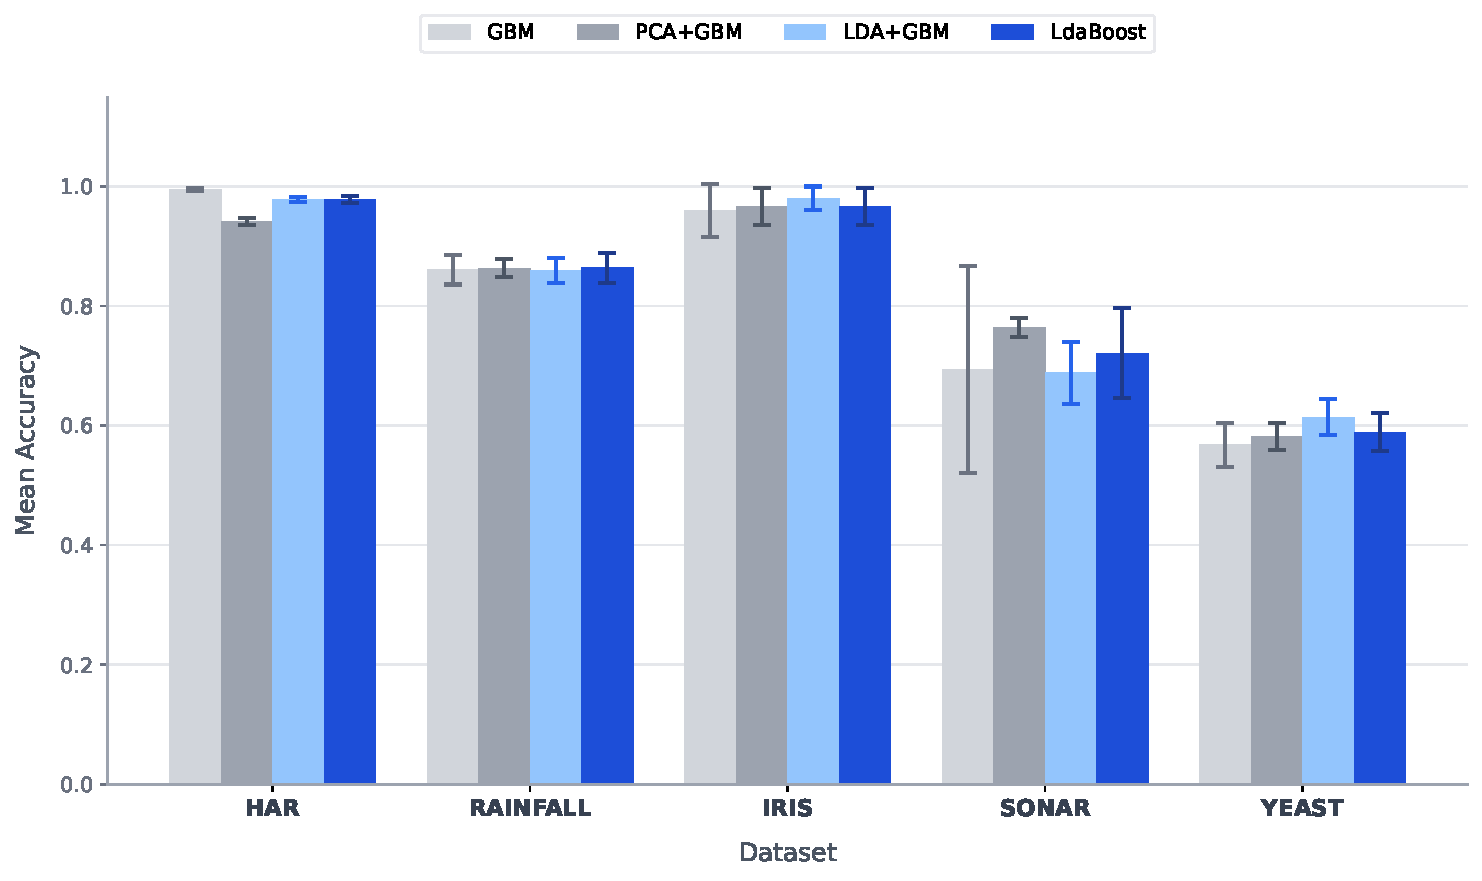
\includegraphics[width=0.75\linewidth]{figures/accuracy_comparison.pdf}
        \caption{\DIFaddFL{Accuracy comparison across real datasets: LDA-based approaches (LDA+GBM and \textsc{LdaBoost}) are most frequently among the best-performing models.}}
        \label{fig:accuracy_comparison_real}
\end{figure}


\DIFaddend \bigskip
\noindent
The Yeast dataset (8 features) showed substantial improvements, with cross-validated accuracy rising from 0.568 (SD = 0.037) for GBM to  \DIFaddbegin \DIFadd{0.614 }\DIFaddend (SD =  \DIFaddbegin \DIFadd{0.030) with }\DIFaddend LDA+GBM \DIFaddbegin \DIFadd{, while LdaBoost reached 0.589 }\DIFaddend (SD =  \DIFaddbegin \DIFadd{0.032}\DIFaddend ) and PCA+GBM  \DIFaddbegin \DIFadd{0.582 }\DIFaddend (SD = 0.023). This confirms the benefit of incorporating discriminant components in multiclass problems even when the feature space is relatively low dimensional.

With a small number of features such as in the IRIS dataset, LDA+GBM delivered the highest accuracy ( \DIFaddbegin \DIFadd{0.980}\DIFaddend , SD =  \DIFaddbegin \DIFadd{0.020}\DIFaddend ). LdaBoost  \DIFaddbegin \DIFadd{and PCA+GBM (both }\DIFaddend 0.967, SD =  \DIFaddbegin \DIFadd{0.031}\DIFaddend ) and GBM (0.960, SD = 0.044) performed similarly .

For the Sonar dataset (binary target, 60 features), the baseline GBM obtained 0.694 (SD = 0.173),  \DIFaddbegin \DIFadd{LDA}\DIFaddend +GBM  \DIFaddbegin \DIFadd{0.688 }\DIFaddend (SD =  \DIFaddbegin \DIFadd{0.052}\DIFaddend ), and  \DIFaddbegin \DIFadd{LdaBoost 0.721 }\DIFaddend (SD =  \DIFaddbegin \DIFadd{0.075), while PCA+GBM }\DIFaddend achieved the best performance at  \DIFaddbegin \DIFadd{0.764 }\DIFaddend (SD =  \DIFaddbegin \DIFadd{0.016)}\DIFaddend . In the Rainfall dataset (binary target, 11 features), performances were comparable, with GBM at 0.861 (SD = 0.025), PCA+GBM at  \DIFaddbegin \DIFadd{0.863 }\DIFaddend (SD =  \DIFaddbegin \DIFadd{0.015}\DIFaddend ), LDA+GBM at  \DIFaddbegin \DIFadd{0.860 }\DIFaddend (SD =  \DIFaddbegin \DIFadd{0.021}\DIFaddend ), and LdaBoost slightly ahead at 0.864 (SD = 0.025).

Regarding test accuracy, for HAR the LDA+GBM model reached  \DIFaddbegin \DIFadd{0.9528, LdaBoost 0.9511, GBM 0.9400}\DIFaddend , and PCA+GBM  \DIFaddbegin \DIFadd{0.9053}\DIFaddend . In the Rainfall dataset \DIFaddbegin \DIFadd{, GBM achieved 0.8790, }\DIFaddend PCA+GBM  \DIFaddbegin \DIFadd{0.8721, }\DIFaddend LDA+GBM  \DIFaddbegin \DIFadd{0.8607, and LdaBoost 0.8584}\DIFaddend .

These findings suggest that the benefits of LdaBoost become increasingly evident as the complexity of the classification task increases, particularly with respect to the number of classes, though not necessarily with feature dimensionality in multiclass settings. In contrast, for binary classification, the added value of LdaBoost tends to grow with higher feature dimensionality. These trends support the overall effectiveness and robustness of the integrated LDA-boosting approach across a range of data scenarios.

\subsection*{Comparative performance of different pipelines: simulations}
 \DIFaddbegin \DIFadd{We first begin }\DIFaddend our simulations with  \DIFaddbegin \DIFadd{a moderate sample size ($N=1{,}000$). }\DIFaddend Figures~\ref{fig:fig1} and~\ref{fig:fig2} illustrate the accuracy trends observed in  multiclass and binary classification scenarios, respectively\DIFaddbegin \DIFadd{, }\DIFaddend as the number of features varies at  \DIFaddbegin \DIFadd{an intermediate mean correlation level ($\rho\approx 0.5$). These figures highlight }\DIFaddend the comparative performance advantages of LdaBoost over classical GBM  \DIFaddbegin \DIFadd{and show that LdaBoost can }\DIFaddend maintain robust predictive accuracy  \DIFaddbegin \DIFadd{as }\DIFaddend feature dimensionality increases .

The simulation results clearly demonstrate that LdaBoost consistently outperformed GBM across varying numbers of features, particularly evident in scenarios with multiclass targets (Figure~\ref{fig:fig1}).


\begin{figure}[h!]
    \centering
    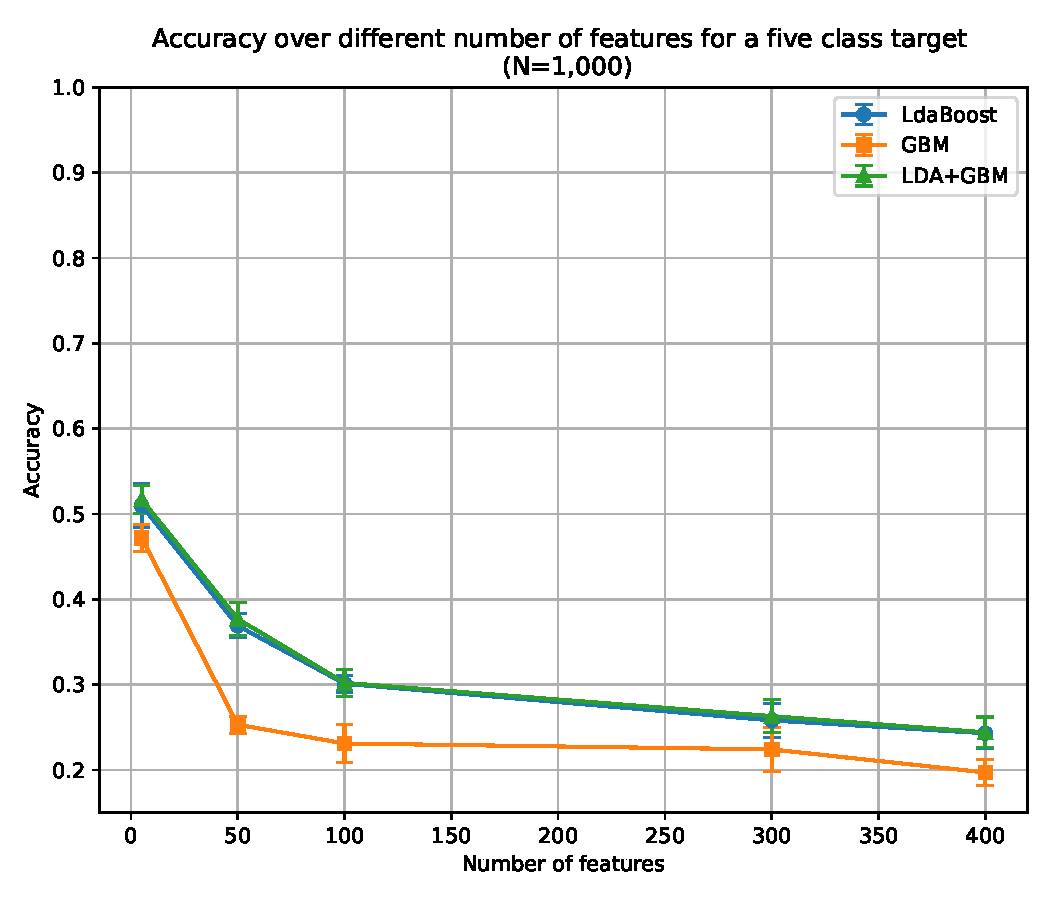
\includegraphics[width=0.6\linewidth]{figures/Accuracy over different number of features for a five class target.pdf}
    \caption{\textit{Accuracy for a multiclass target as a function of the number of features ($\rho\approx0.5$)}}
    \label{fig:fig1}
\end{figure}

As the number of features increased, both LdaBoost and LDA+GBM consistently outperformed the standard GBM model, with particularly notable accuracy gains in the 50–100 feature range. This highlights the effectiveness of LDA-based feature extraction. Moreover, the performance gap between GBM and the two LDA-integrated methods remained relatively stable, emphasizing the advantage of combining discriminant analysis with boosting in high-dimensional classification settings.

A similar pattern emerged in the binary classification setting (Figure~\ref{fig:fig2}): although performance differences were less pronounced, LdaBoost continued to outperform GBM, especially at intermediate levels of feature dimensionality (around 50–100 features). However, as dimensionality increased further ($p > 270$), the accuracy of the two methods tended to converge.

\begin{figure}[h!]
    \centering
    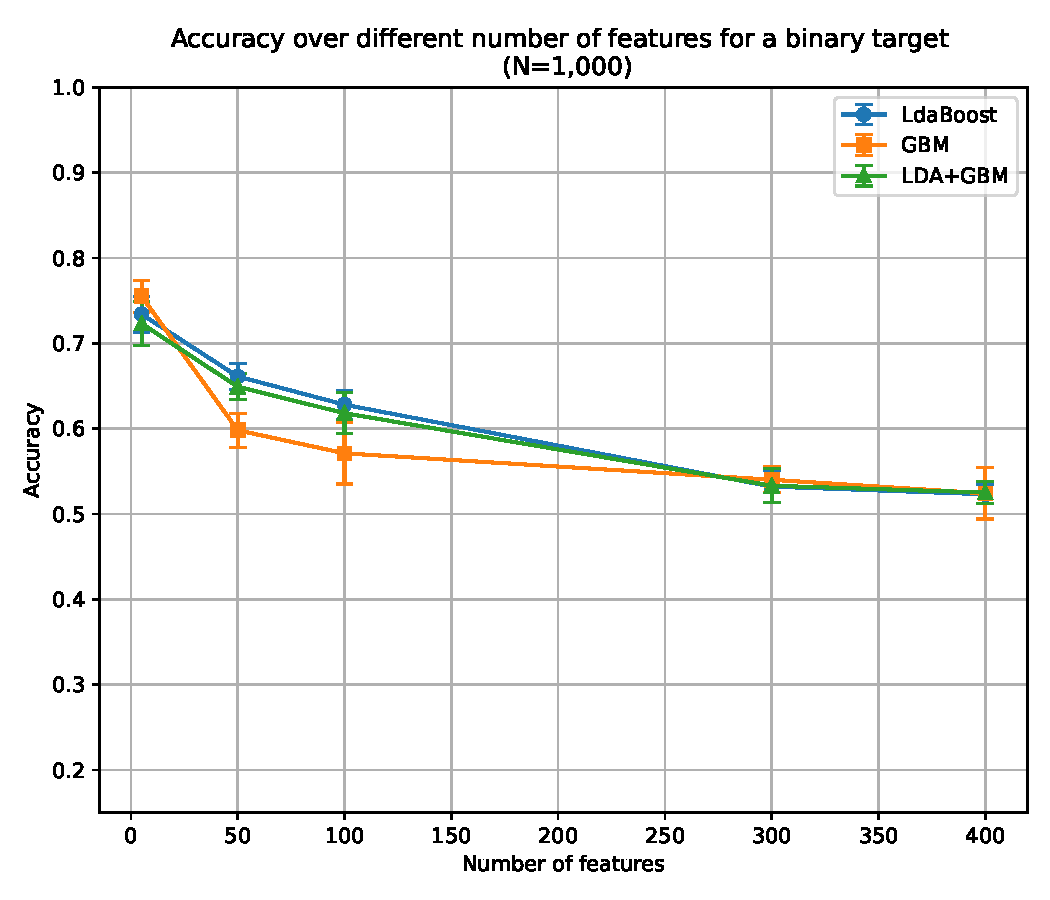
\includegraphics[width=0.6\linewidth]{figures/Accuracy over different number of features for a binary target.pdf}
    \caption{\textit{Accuracy for a binary target as a function of the number of features ($\rho\approx0.5$)}}
    \label{fig:fig2}
\end{figure}

Notably, in both binary and multiclass settings, LDA+GBM closely mirrored the performance trajectory of LdaBoost. In the binary case, LdaBoost consistently outperformed LDA+GBM, particularly at moderate levels of feature dimensionality, suggesting that in more complex feature spaces, LDA-based feature extraction alone can significantly enhance the predictive power of boosting methods. 

\DIFaddbegin \DIFadd{For binary targets, this behavior is noteworthy because $C=2$ implies that each LDA fit yields only one discriminant component. Consequently, each boosting stage is trained on a one-dimensional score, and LdaBoost's competitiveness comes from repeatedly updating that score direction across rounds rather than from a high-dimensional transformed representation. This also clarifies why the method is conceptually strongest in multiclass settings, where $C-1$ provides a richer discriminant subspace.
}

\DIFaddend These results are systematically the same over other mean levels of correlations among features (Figure~\ref{fig:fig7} and Figure~\ref{fig:fig8} in the Appendix). Particularly, the added value of LdaBoost (and LDA+GBM) over GBM increases when the mean correlation increases (Figure~\ref{fig:fig8}). 

With an increased number of observations, Figure~\ref{fig:A7} in the Appendix replicates Figure~\ref{fig:fig2} (binary target) for N = 10,000, showing that the two newly introduced algorithms continue to outperform GBM across all feature sets—unlike in the  \DIFaddbegin \DIFadd{N = 1,000 }\DIFaddend case, where the performance gap disappeared for larger numbers (270-300) of features.

\DIFaddbegin \subsection*{\DIFadd{Runtime-ablation evidence}}
\DIFadd{To complement the complexity discussion in Section 3, we performed a runtime ablation with fixed seeds over two synthetic scenarios: a high-dimensional binary task ($N=1200$, $p=300$, $\rho=0.5$) and a multiclass task ($N=1200$, $p=100$, $C=5$, $\rho=0.5$). For each scenario we repeated the train/test experiment five times and compared GBM, PCA+GBM, LDA+GBM (one-shot transform), and LdaBoost (dynamic per-round LDA).
}

\DIFadd{Table~\ref{tab:runtime_ablation} reports mean fit time and test accuracy with standard deviations. In the binary high-dimensional setting, LdaBoost has fit time close to GBM and much larger than one-shot LDA+GBM, consistent with the expected iterative-LDA overhead. In the multiclass setting, LdaBoost remains slower than one-shot LDA+GBM but faster than GBM. Since these ablation runs use fixed hyperparameters and prioritize computational comparison, their accuracy values should be interpreted as runtime-context evidence rather than as tuned performance ceilings. Overall, the experiment empirically confirms the runtime-accuracy trade-off implied by stagewise LDA updates.
}

\begin{table}[h!]
\centering
\begingroup
\setlength{\tabcolsep}{4.5pt}
\renewcommand{\arraystretch}{1.0}
\footnotesize
\caption{\DIFaddFL{Runtime ablation on synthetic scenarios (5 seeds): fit time in seconds and test accuracy, reported as mean (SD).}}
\label{tab:runtime_ablation}
\begin{tabular}{@{}llcc@{}}
\toprule
\DIFaddFL{\textbf{Scenario} }& \DIFaddFL{\textbf{Model} }& \DIFaddFL{\textbf{Fit Time (s)} }& \DIFaddFL{\textbf{Test Accuracy} }\\
\midrule
\multirow{4}{*}{\textbf{Binary, $p=300$}}
    & \DIFaddFL{GBM      }& \DIFaddFL{2.702 (0.025) }& \DIFaddFL{0.770 (0.032) }\\
    & \DIFaddFL{PCA+GBM  }& \DIFaddFL{0.506 (0.012) }& \DIFaddFL{0.761 (0.035) }\\
    & \DIFaddFL{LDA+GBM  }& \DIFaddFL{0.077 (0.014) }& \DIFaddFL{0.685 (0.018) }\\
    & \DIFaddFL{LdaBoost }& \DIFaddFL{2.683 (0.105) }& \DIFaddFL{0.681 (0.020) }\\
\midrule
\multirow{4}{*}{\textbf{Multiclass, $p=100$}}
    & \DIFaddFL{GBM      }& \DIFaddFL{4.497 (0.054) }& \DIFaddFL{0.591 (0.026) }\\
    & \DIFaddFL{PCA+GBM  }& \DIFaddFL{1.312 (0.012) }& \DIFaddFL{0.586 (0.018) }\\
    & \DIFaddFL{LDA+GBM  }& \DIFaddFL{0.365 (0.005) }& \DIFaddFL{0.536 (0.028) }\\
    & \DIFaddFL{LdaBoost }& \DIFaddFL{1.153 (0.010) }& \DIFaddFL{0.541 (0.033) }\\
\bottomrule
\end{tabular}
\endgroup
\end{table}

\DIFaddend \subsection*{LdaBoost Simulations}
To deeply assess how LdaBoost works in different scenarios, this subsection provides further insight into how LdaBoost accuracy varies.

Analyzing  \DIFaddbegin \DIFadd{first the role of mean }\DIFaddend feature correlation $\rho$ \DIFaddbegin \DIFadd{with $N=1{,}000$ observations}\DIFaddend , the binary simulations reveal that higher correlations ($\rho = 0.7$) deliver the highest accuracies when the feature space is moderately sized, reaching mean values around 0.80 at $p = 5$ and $p = 50$. At $\rho = 0.3$, accuracies lie between 0.59 and 0.77, whereas under no correlation ($\rho = 0.0$) they remain between 0.55 and 0.69. As dimensionality increases towards $p = 400$, the advantage of highly correlated features diminishes and the mean accuracy falls back to roughly 0.63, consistent with the onset of the Hughes phenomenon.

Figure~\ref{fig:fig3} illustrates how LdaBoost accuracy varies over both the number of features and $\rho$ in a binary classification task, also in comparison with accuracy of the optimal Bayes classifier. The model benefits the most from 50--100 features when correlations are moderate or high, while strong correlations become detrimental once $p$ exceeds roughly 200. In contrast, under $\rho \approx 0$ the curves are flatter, with modest gains up to 300 features before a slight decline.

These results suggest that in  \DIFaddbegin \DIFadd{this finite-sample regime }\DIFaddend LdaBoost capitalizes on redundant information when dimensionality is controlled, but still faces the usual degradation as $N/p$ shrinks. When features are effectively independent, increases in dimensionality yield only incremental improvements, confirming that the architecture remains sensitive to the balance between sample size and feature count.


\begin{center}
\begin{figure}[h!]
    \centering
    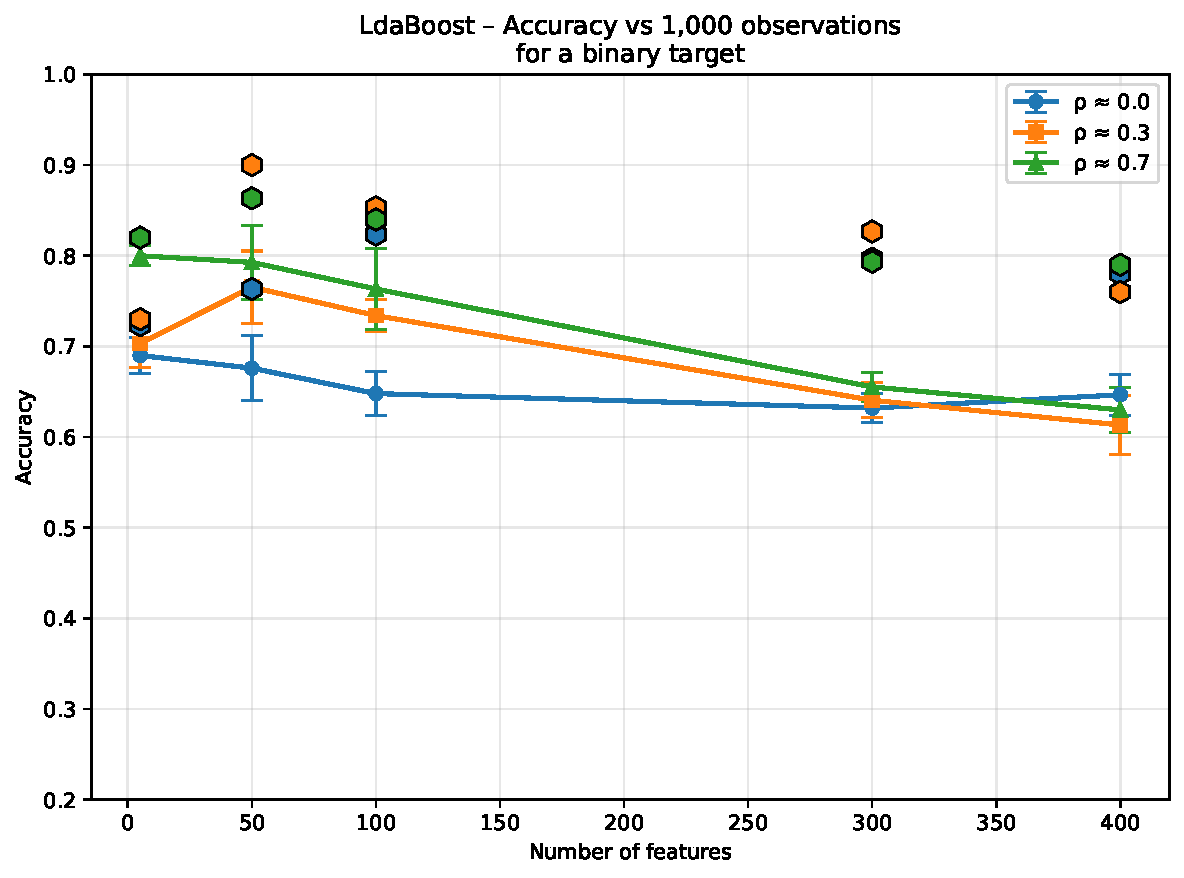
\includegraphics[width=0.6\linewidth]{figures/ldaboost_accuracy_binary_1k.pdf}
    \caption{\textit{LdaBoost accuracy by number of features and average correlation levels ($\rho$): binary target. Points indicate the accuracy of the Bayes classifier.}}
    \label{fig:fig3}
\end{figure}

\begin{figure}[h!]
    \centering
    \begin{subfigure}{0.6\linewidth}
        \centering
        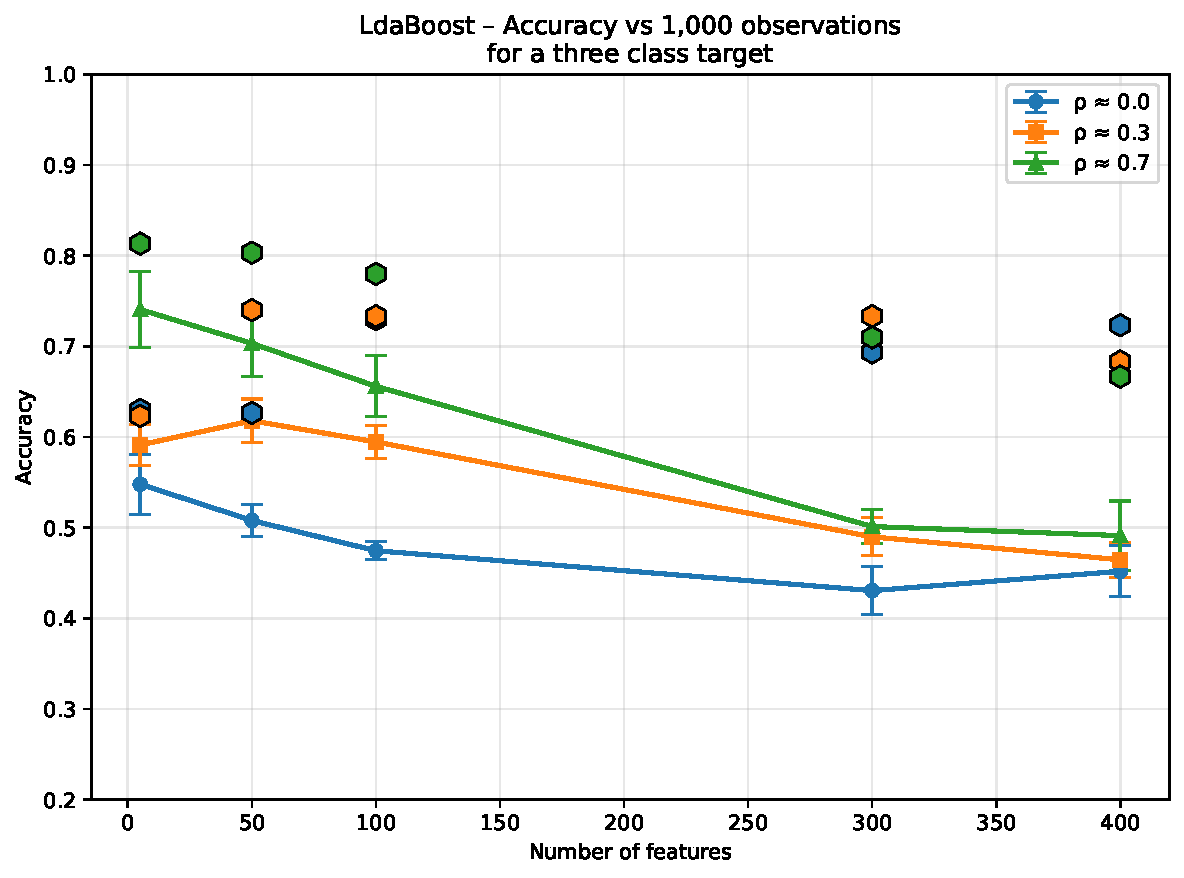
\includegraphics[width=\linewidth]{figures/ldaboost_accuracy_three class_1k.pdf}
        \caption{3 classes}
    \end{subfigure}

    \begin{subfigure}{0.6\linewidth}
        \centering
        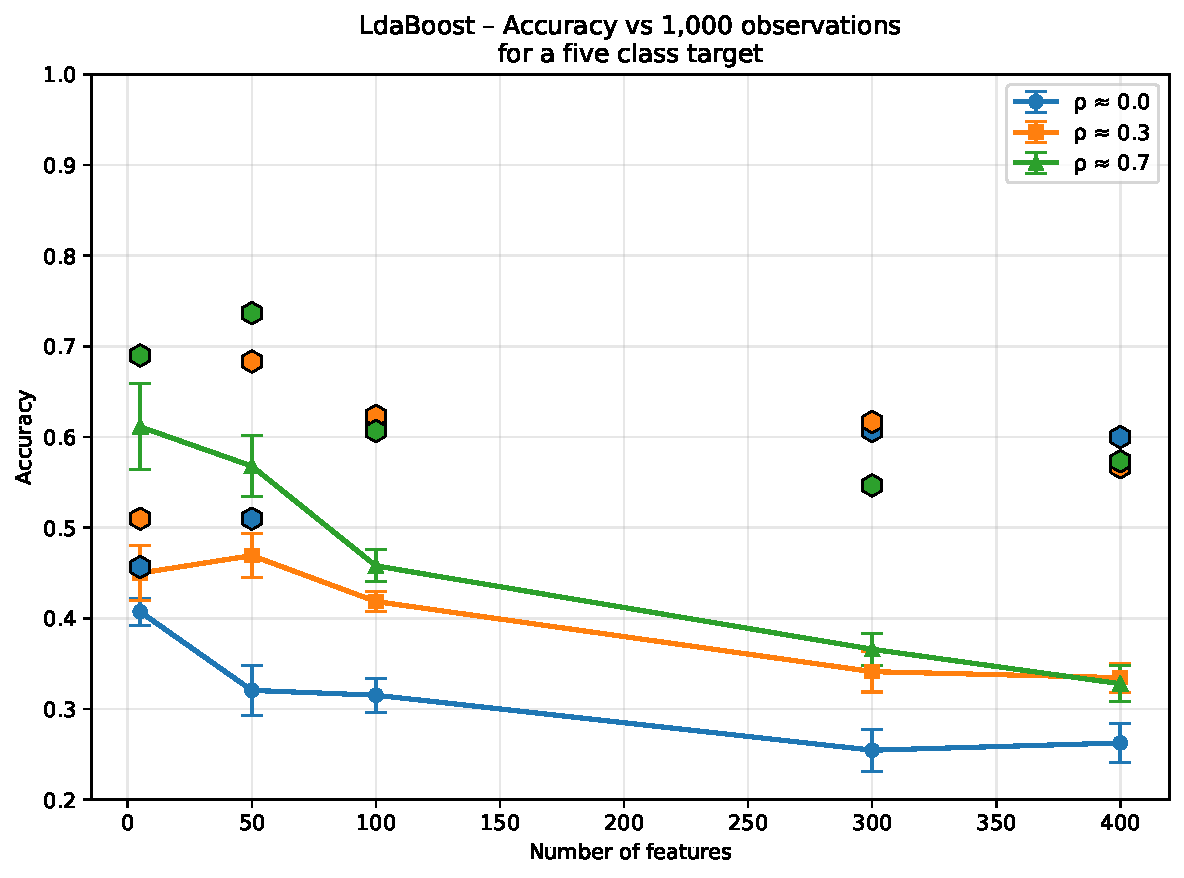
\includegraphics[width=\linewidth]{figures/ldaboost_accuracy_multiclass_1k.pdf}
        \caption{5 classes}
    \end{subfigure}\\[2ex]
    \caption{\textit{LdaBoost accuracy by number of features and average correlation levels ($\rho$): multiclass target: 3 classes (top), 5 classes (bottom). Points indicate the accuracy of the Bayes classifier.}}
    \label{fig:fig4}
\end{figure}
\end{center}

\newpage
Figure~\ref{fig:fig4} illustrates how accuracy varies for multiclass targets with 3 (top) and 5 classes (bottom). The main finding is that, in all scenarios, accuracy is higher for binary targets and decreases as the number of classes increases. Moreover, as the number of covariate increases, the accuracies tend to converge to the same value regardless of the level of correlation, and this effect is more pronounced when the target variable has fewer classes.

This may be a clear finding of the so-called Hughes phenomenon \citep{hughes1968mean}, shown here for binary targets. The core idea is that as the number of features increases, the classification accuracy of statistical pattern recognizers does not necessarily improve—and may even decline or stabilize—especially when the number of training samples is limited. In fact, data become sparse in high dimensions, and the classifier has fewer observations per unit volume of the feature space to estimate class boundaries reliably. Hughes showed that there is an optimal number of features for a given sample size and classifier type. Beyond that point, adding more features does not improve and may harm classification accuracy.

This effect is more pronounced when the features are highly correlated or when the sample size is low relative to the number of features. Figures~\ref{fig:fig3} and ~\ref{fig:fig4} clearly illustrate both effects, especially the sharp decline in accuracy for high levels of feature correlation. Moreover, regarding the latter aspect, given that the sample size ($N$) is always fixed at 1000, for a large number of features ($p$), the ratio $N/p$ declines substantially. This Hughes phenomenon is less marked when the number of classes increases (Figure~\ref{fig:fig4}) 
Moreover, Figures~\ref{fig:fig5} and ~\ref{fig:fig6} illustrate simulation results with 10,000 observations for multiclass (5 classes) and binary target, respectively. These pictures highlight that, as expected, large samples mitigate the Hughes effect, especially for the binary target.\\[2ex]
The large sample experiment ($N = 10{,}000$) confirms that LdaBoost tracks the optimal Bayes estimator remarkably closely in the multiclass setting (Figure~\ref{fig:fig5}). Differences are quite stable, with the smallest gaps observed when the dependence structure strengthens. 

An improved pattern emerges for the binary target (Figure~\ref{fig:fig6}). LdaBoost holds its Bayes-level accuracy for more than 100 features and even benefits from growing correlation, which slightly narrows the residual gap to the optimal Bayes estimator before the Hughes effect eventually dampens both models beyond that threshold.
This behavior suggests that, in the binary case, the discriminant projections within the boosting loop capture nearly all of the Bayes-optimal separation in moderately high-dimensional settings, such as those where researchers typically work with a few dozen informative, correlated covariates.

\begin{figure}[h!]
    \centering
    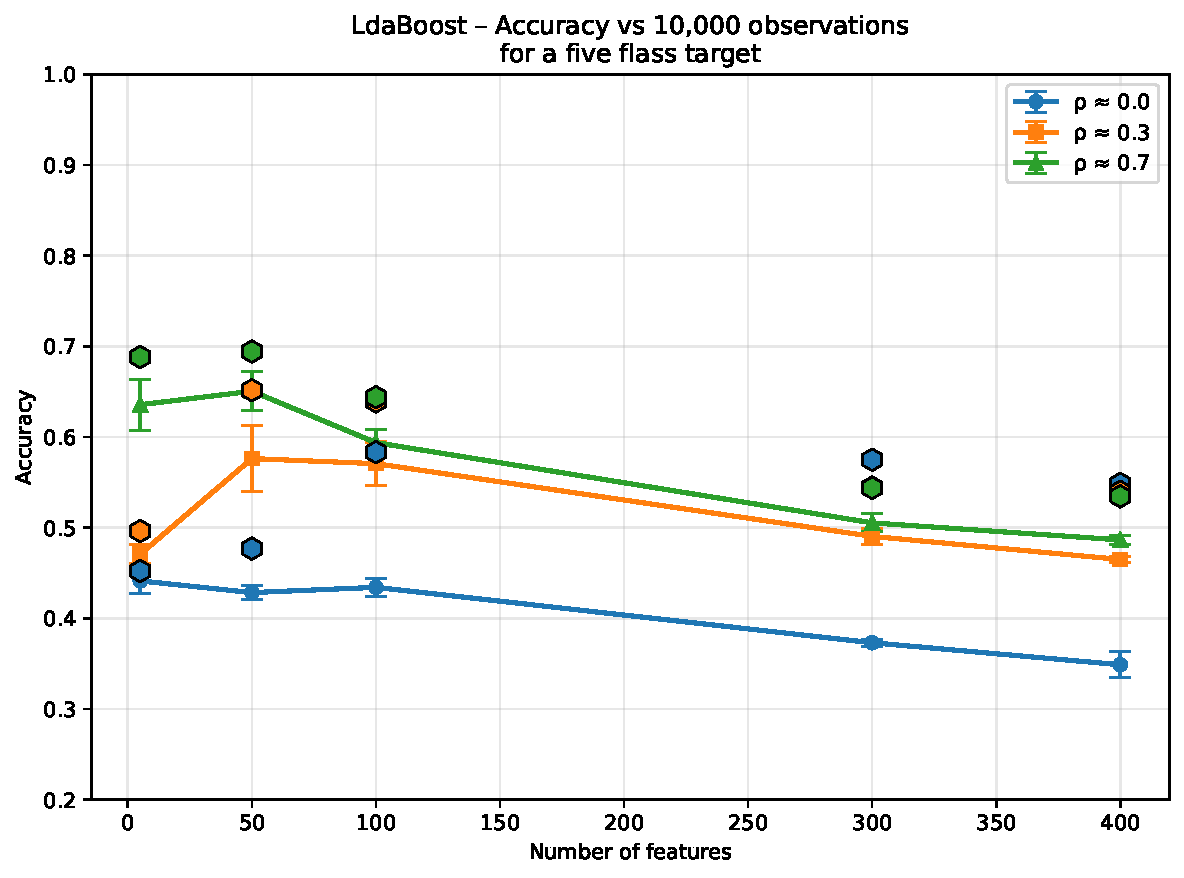
\includegraphics[width=0.6\linewidth]{figures/ldaboost_accuracy_multiclass_10k.pdf}
    \caption{Accuracy over 10,000 observations
for a five class target}
    \label{fig:fig5}
\end{figure}
\begin{figure}[h!]
    \centering
    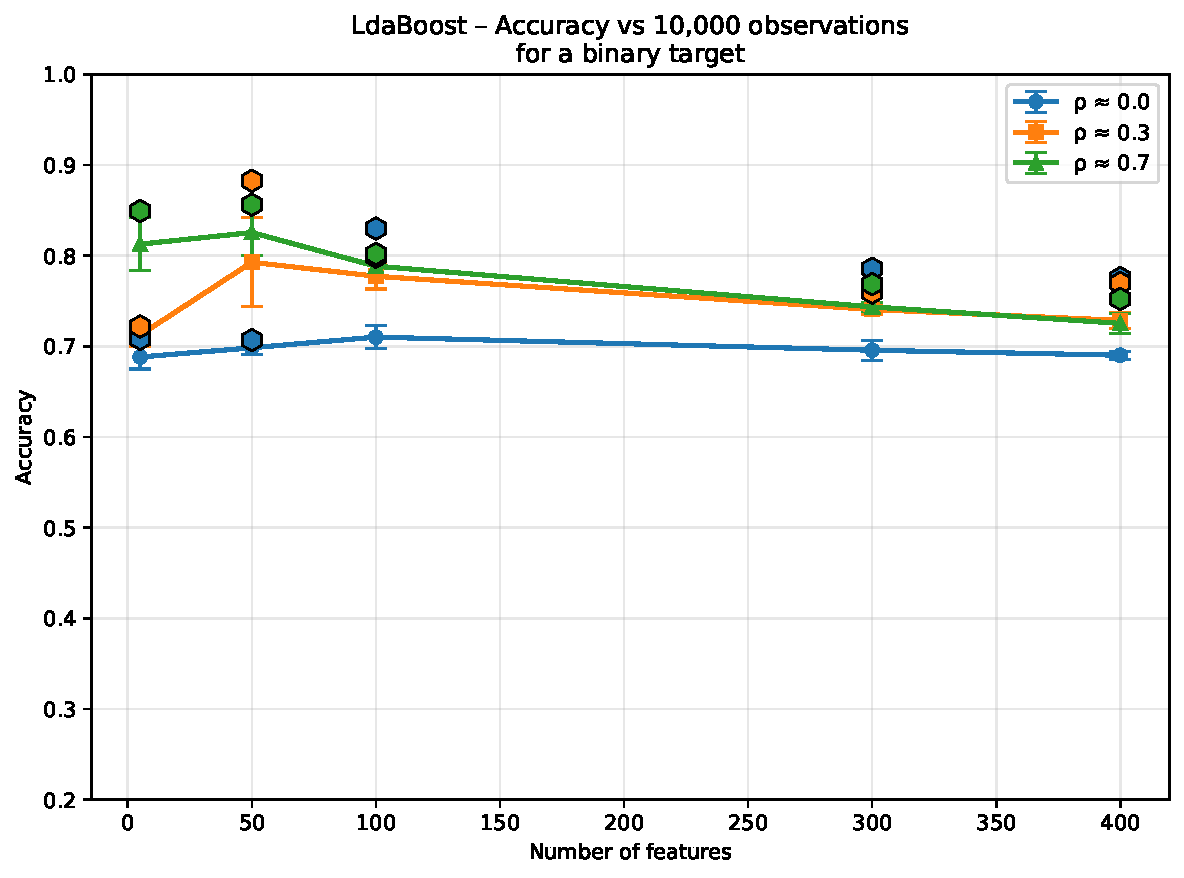
\includegraphics[width=0.6\linewidth]{figures/ldaboost_accuracy_binary_10k.pdf}
    \caption{Accuracy over 10,000 observations
for a binary target}
    \label{fig:fig6}
\end{figure}

\section{Conclusion}
To our knowledge, no previous study has investigated the use of LDA in conjunction with gradient boosting. Specifically, there is no established practice or empirical evidence suggesting that LDA enhances performance or is inherently compatible with gradient boosting models. Beyond analyzing the effects of PCA and LDA as feature extraction techniques on the accuracy of gradient boosting machines, we propose an integrated iterative algorithm—LdaBoost—that applies LDA-based feature transformation at each boosting iteration.

Empirically, we compare the classification performance of standard GBM with PCA, GBM with LDA preprocessing, and the proposed LdaBoost algorithm across five benchmark datasets. In most cases, LdaBoost or GBM with LDA preprocessing improved on standard GBM in cross-validated and test accuracy, the HAR dataset being the unique case demonstrating that baseline GBM can still be competitive when all features are retained.

Overall, the results show that LdaBoost \DIFaddbegin \DIFadd{often }\DIFaddend yields increased performance gains as classification tasks become more complex in terms of the number of target classes. However, this pattern is less pronounced when the number of features is increased in multiclass settings. In contrast, in binary classification tasks, LdaBoost exhibits a clear advantage as the dimensionality of the features increases \DIFaddbegin \DIFadd{in the main tuned analyses}\DIFaddend . These findings highlight the adaptability and robustness of the LDA-boosting framework across a variety of data structures.

Simulation studies indicate improved accuracy in binary classification under moderate feature complexity and high feature correlation, and also clearly reveal the presence of the Hughes phenomenon (curse of dimensionality).

Together, these insights underscore LdaBoost’s robust adaptability to different data conditions, demonstrating its practical utility in diverse classification scenarios, particularly in settings characterized by high dimensionality and substantial feature correlation\DIFaddbegin \DIFadd{. The runtime-ablation analysis also shows that these gains come with measurable computational overhead versus one-shot LDA preprocessing, so the practical choice depends on the target balance between accuracy and training cost}\DIFaddend . In particular, the comparison with the optimal Bayes estimator (especially for the $N=10{,}000$ simulations and binary target) shows that LdaBoost stays virtually coincident with the Bayes-optimal curve for more than 100 correlated covariates, demonstrating that the method preserves near-optimal discrimination in the most relevant feature ranges.

\newpage
\section*{Appendix}
\appendix
\renewcommand{\thefigure}{A\arabic{figure}}
\begin{figure}[h!]
    \centering
    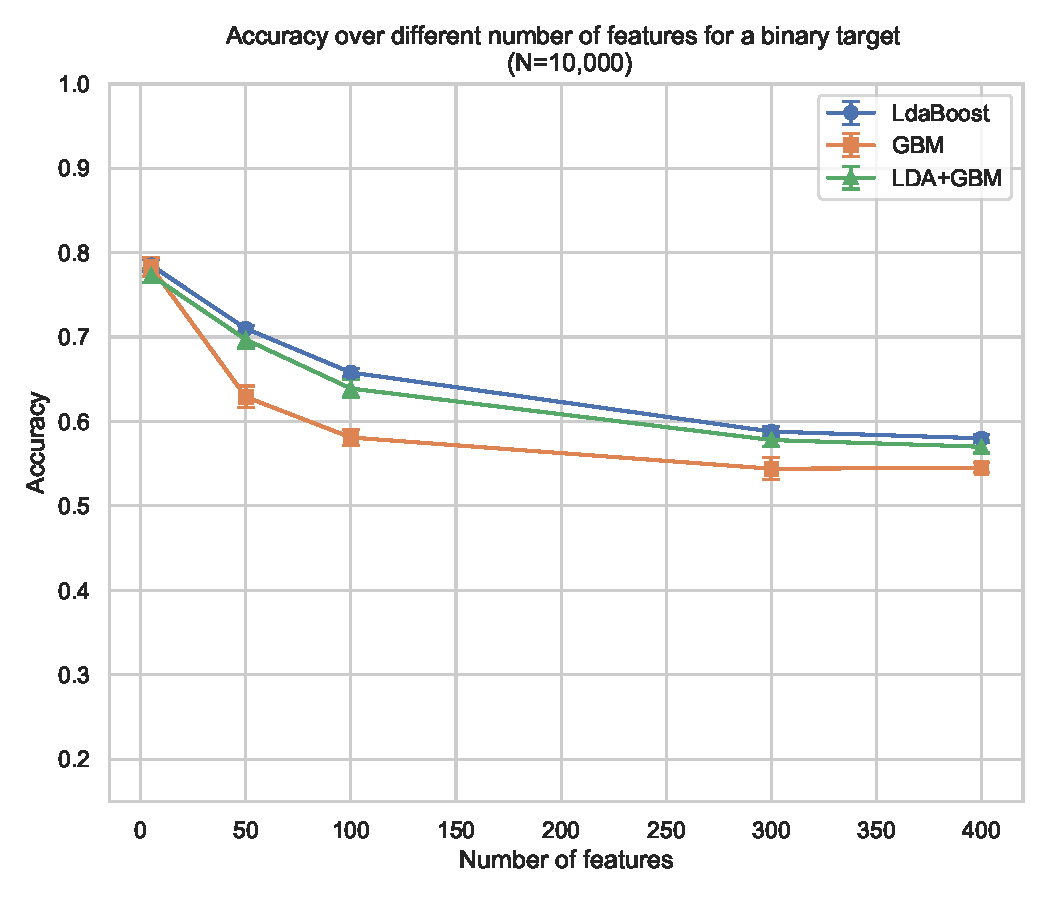
\includegraphics[width=0.6\linewidth]{figures/Accuracy over different number of features for a binary target (N=10,000).pdf}
    \caption{\textit{Accuracy for a binary target as a function of the number of features ($\rho\approx0.5$)}}
    \label{fig:A7}
\end{figure}
\begin{figure}[h!]
    \centering
    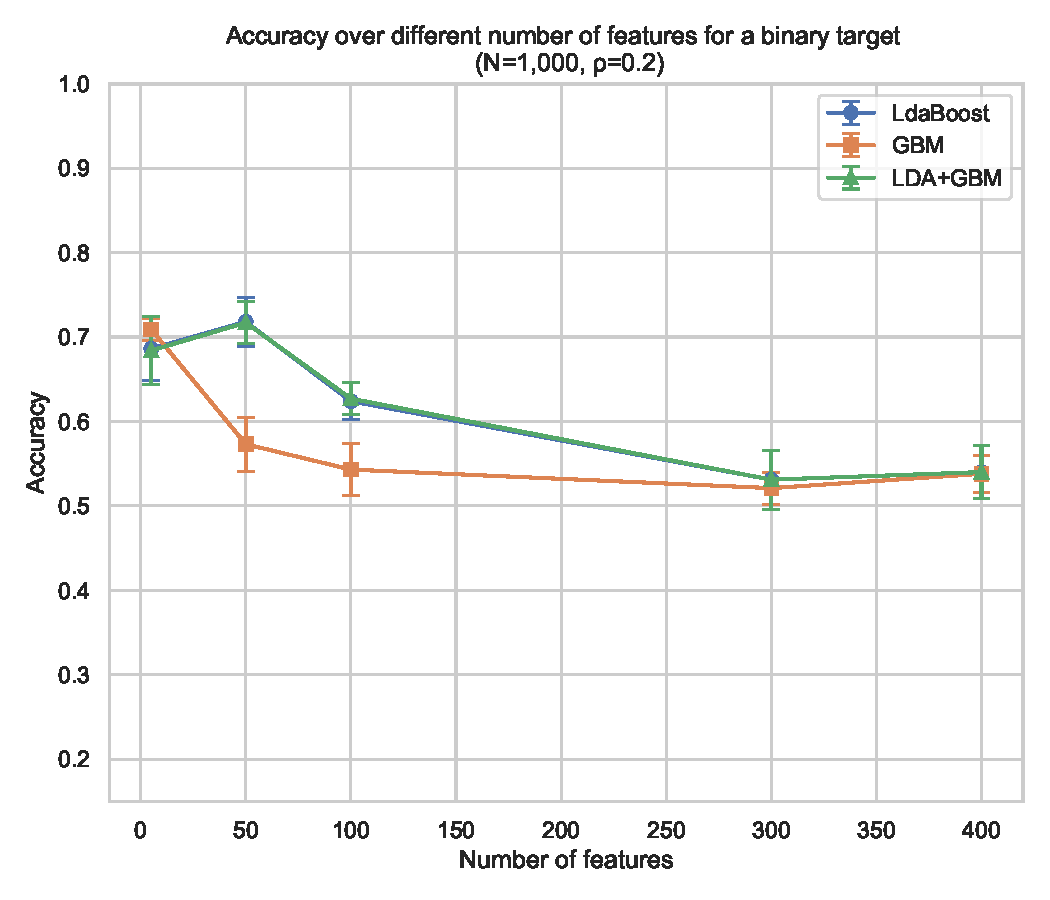
\includegraphics[width=0.6\linewidth]{figures/Accuracy over different number of features for a binary target low correlation.pdf}
    \caption{Confronting the different pipelines in a low correlation scenario.}
    \label{fig:fig7}
\end{figure}
\begin{figure}[h!]
    \centering
    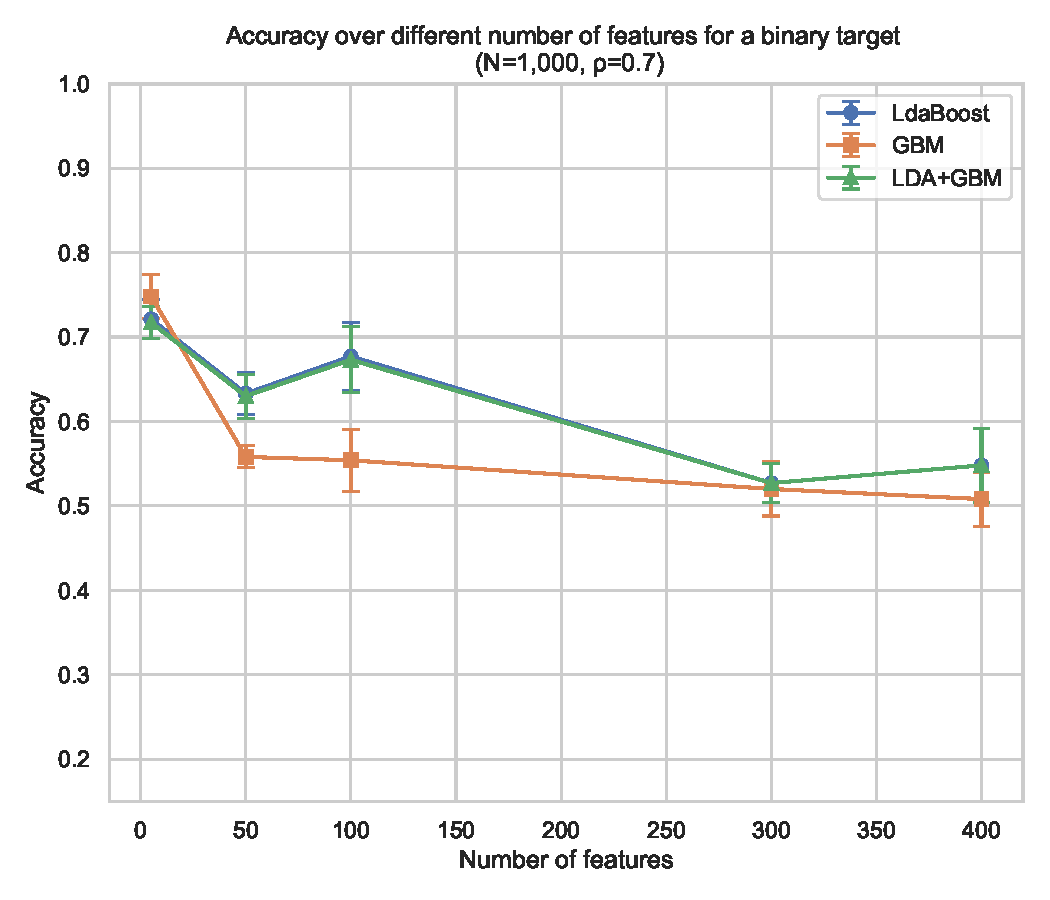
\includegraphics[width=0.6\linewidth]{figures/Accuracy over different number of features for a binary target high correlation.pdf}
    \caption{Confronting the different pipelines in a high correlation scenario.}
    \label{fig:fig8}
\end{figure}






\newpage
\bibliographystyle{plainnat}
\bibliography{references}

\end{document}
